\documentclass{cam-thesis}

%%%%%%%%%%%%%%%%%%%%%%%%%%%%%%%%%%%%%%%%%%%%%%%%%%%%%%%%%%%%%%%%%%%%%%%%%%%%%%%%
%% Packages
%%%%%
\usepackage[british]{babel}
\usepackage[numbers,sort&compress]{natbib}
\usepackage{amsmath}
\usepackage{amssymb}
\usepackage{graphicx}
\usepackage{booktabs}
\usepackage{hyperref}
\usepackage{microtype}
\usepackage{subcaption}
\usepackage{xcolor}
\usepackage{multirow}

%%%%%%%%%%%%%%%%%%%%%%%%%%%%%%%%%%%%%%%%%%%%%%%%%%%%%%%%%%%%%%%%%%%%%%%%%%%%%%%%
%% Thesis meta-information
%%%%%
\title{Automated Detection of Satellite Trails in Ground-Based Observations
       Using U-Net and the Probabilistic Hough Transform}

\author{Baron Gracias}

\college{Clare College}

\collegeshield{CollegeShields/Clare}

\departments{Department of Physics (Cavendish Laboratory)\\
             Institute of Astronomy}

\degree{MPhil Data Intensive Science}

\supervision{Dr Eduardo Gonzalez-Solares}

\submissionnotice{This dissertation is submitted for the degree of Master of
                  Philosophy in Data Intensive Science}

\date{July 2026}

% Word count per Course Handbook 4.3.2: includes summary/abstract, tables,
% footnotes, and non-auto-generation appendices; excludes table of contents,
% equations, figure captions, bibliography, and the auto-generation appendix.
% Handbook basis ~6,950 with section headings excluded (texcount body ~6,595
% + abstract ~175 + table cells ~255 - auto-generation appendix 75).
\wordcount{6950}

\subjectline{Data Intensive Science}
\keywords{satellite trails, U-Net, Hough transform, deep learning, MeerLICHT,
          binary segmentation, astronomical image processing}

%% Declaration page omitted: the example DIS report carries no originality
%% declaration, and the 7,000-word limit is tracked at submission instead.
\declaration{}

%%%%%%%%%%%%%%%%%%%%%%%%%%%%%%%%%%%%%%%%%%%%%%%%%%%%%%%%%%%%%%%%%%%%%%%%%%%%%%%%
%% Abstract (concise framing only; headline metrics are deferred to drafting)
%%%%%
\abstract{%
  The proliferation of low-Earth-orbit satellite constellations has made
  automated detection and masking of satellite trails a routine requirement for
  wide-field observatories.
  %
  This dissertation replicates the U-Net plus probabilistic Hough transform
  pipeline of \citet{stoppa2024} on a labelled MeerLICHT subset. The PyTorch
  implementation uses an architecture-faithful U-Net, a combined binary
  cross-entropy and squared-Dice loss, validation-only model and threshold
  selection, and Hough post-processing of the probability map. The replication is
  then examined through four analyses: residual error, model variants,
  training-protocol sensitivity, and inference-time strategies.
  %
  The replication reproduces the paper's recall (five-seed test recall $0.923$
  against $0.94$) and its Hough completeness (trail-pixel recall
  $0.918\rightarrow0.990$; a pixel-level false-negative rate
  $0.082\rightarrow0.0105$ comparable to the paper's
  $6.98\,\%\rightarrow3.38\,\%$), while strict pixel precision sits below the
  paper and is prevalence-dependent.
  %
  The residual-error analysis narrows the gap: $82.5\,\%$ of false positives
  fall in trail-bearing patches, and separate tolerance and distance diagnostics
  place much of the residual within one pixel of the mask.
  A blinded single-author re-annotation of $64$ sealed crops finds no systematic
  width bias between the original masks, the re-annotation, and the model.
  Model, training, and inference variants move the residual only slightly. The
  evidence therefore supports a narrow conclusion: recall and Hough completeness
  reproduce, while the remaining strict-precision gap is most consistent with
  boundary-scale annotation disagreement on this dataset.
}


%%%%%%%%%%%%%%%%%%%%%%%%%%%%%%%%%%%%%%%%%%%%%%%%%%%%%%%%%%%%%%%%%%%%%%%%%%%%%%%%
\begin{document}

\frontmatter{}

%%%%%%%%%%%%%%%%%%%%%%%%%%%%%%%%%%%%%%%%%%%%%%%%%%%%%%%%%%%%%%%%%%%%%%%%%%%%%%%%
%% CHAPTER 1 -- Introduction and context
%% Scope: motivate the problem (constellation growth, survey contamination),
%% introduce the target paper, state aims/scope/contributions, and outline the
%% dissertation. Context and brief related work live here.
%%%%%
\chapter{Introduction and Context}
\label{ch:introduction}

The low-Earth-orbit satellite population is growing quickly. CelesTrak listed
15{,}848 active satellites on 27 May 2026, of which approximately 14{,}600
occupied orbits below 2{,}000\,km, including more than 10{,}000 Starlink
spacecraft \citep{celestrak2026}. Regulatory approvals extend further:
15{,}000 second-generation Starlink satellites are approved \citep{fcc2026}, and
policy reviews treat proposals exceeding 100{,}000 spacecraft as realistic
\citep{walker2020,walker2021}. Each sunlit satellite crossing a wide-field
exposure leaves a bright, near-linear trail that corrupts photometry and
astrometry along its path and injects spurious candidates into
transient-detection pipelines \citep{tyson2020,hainaut2020}.

The contamination is already measurable. Starlink trails affected under
$0.5\,\%$ of Zwicky Transient Facility twilight images in late 2019 but
$18\,\%$ by August 2021 \citep{mroz2022}; Rubin Observatory simulations
indicate that approximately $10\,\%$ of LSST images would contain at least one
trail under a 40{,}000-satellite scenario \citep{rubin2026}. Other wide-field
twilight exposures can reach $30$--$40\,\%$ contamination
\citep{hainaut2020,bassa2022}, and $4.3\pm0.4\,\%$ of Hubble ACS/WFC images
taken in 2018--2021 contained trails \citep{kruk2023}. At these
rates manual flagging does not scale: a survey instrument such as MeerLICHT
\citep{bloemen2016} produces $10{,}560\times10{,}560$-pixel frames throughout
the night, so identifying and masking affected pixels must be automated,
reliable at the pixel level, and cheap enough to run inside the reduction
pipeline.

\section{The target pipeline}
\label{sec:target_pipeline}

\citet{stoppa2024} present ASTA, the pipeline replicated in this
dissertation: a U-Net \citep{ronneberger2015} trained on manually annotated
MeerLICHT images, followed by a probabilistic Hough transform
\citep{hough1962,matas2000} applied to the network's output probability map.
The two stages serve complementary roles. The U-Net supplies per-pixel soft
detection that survives the crowded stellar background. The Hough stage exploits
the one prior the network does not encode explicitly, that a satellite trail is
globally linear, to connect fragmented detections and extend partially recovered
trails. The published pipeline reaches precision
and recall both approaching $0.94$ and was applied at scale to around
200{,}000 full MeerLICHT fields. The published behaviour is summarised in
Section~\ref{sec:related_target}; the replication results are reported in
Chapter~\ref{ch:analysis}.

\section{Background and related work}
\label{sec:related}


\subsection{Classical trail detection}
\label{sec:related_classical}

Classical satellite-trail detection usually treats trails as geometric line
features. Hough and Radon-family methods map image pixels into line-parameter
space, making them natural tools for long, straight artefacts
\citep{hough1962,duda1972,matas2000}. Astronomical uses include survey
cleaning, masked-star validation in crowded fields, faint-streak matched
filtering, space-debris and {DECam} workflows, and Hubble ACS trail recovery
\citep{storkey2004,bektesevic2017,nir2018,virtanen2016,serrano2026,stark2026}.
Their shared limitation is sensitivity to faint, fragmented, or
background-confused trails, where reliable voting and instrument-specific
preprocessing become difficult; this motivates learned segmentation before
geometric post-processing.

\subsection{Deep learning for astronomical segmentation}
\label{sec:related_dl}

The U-Net architecture \citep{ronneberger2015}, an encoder--decoder with skip
connections that preserve spatial resolution, was designed for biomedical
segmentation and is now common in astronomical imaging. Close precedents for
thin, sparse artefacts are deepCR \citep{zhang2020} and Cosmic-CoNN
\citep{xu2023}, both cosmic-ray segmentation systems. MaxiMask
\citep{paillassa2020} covers contaminant masking including satellite and
aircraft trails, and trails have since been targeted with U-Net plus
line-segment detection \citep{chen2025}, multi-band attention U-Nets
\citep{yu2025}, and end-to-end streak cataloguing \citep{carrillo2026}. No
published trail-detection pipeline was found that gates a segmentation U-Net
with a lightweight patch classifier, although classifiers are already used
elsewhere in the MeerLICHT ecosystem \citep{hosenie2021}.
Section~\ref{sec:ext_twostage} therefore treats this as a narrow follow-up test.

\subsection{The target pipeline: Stoppa et al.\ (2024)}
\label{sec:related_target}

\citet{stoppa2024} trained a U-Net on $528\times528$ MeerLICHT patches with a
combined binary cross-entropy and Dice loss, and applied a probabilistic
Hough transform to the U-Net probability map as a post-processing step. On a
20{,}000-patch test set at threshold $0.58$ the pipeline reported precision and
recall both approaching $0.94$, with the Hough step reducing the pixel-level
false-negative rate from $6.98\,\%$ to $3.38\,\%$. The paper does not report the
training hyperparameters, making faithful replication a non-trivial
search (Chapter~\ref{ch:pipeline}).

\section{Aims, scope, and contributions}
\label{sec:aims}

This dissertation has three aims. The first is a faithful PyTorch replication
of the \citet{stoppa2024} pipeline on the labelled MeerLICHT subset, with the
network architecture reconstructed from the released Keras \texttt{model-best.h5}
file, not the
paper's text alone, and with model and threshold selection locked on
validation data before any test metric is inspected. The second is to
diagnose the residual error of that replication: to establish where the
strict precision gap against the published figures comes from, rather than to
report it as a single number. The third is to test which interventions can
move that residual, through model variants, training-protocol changes, and
inference-time strategies.

The contributions are:
\begin{itemize}
  \item an architecture-faithful, validation-locked replication that
        reproduces the paper's recall and Hough pixel completeness
        (Chapter~\ref{ch:analysis});
  \item a residual-error characterisation that localises the strict precision
        gap at the one-pixel boundary scale;
  \item controlled tests of a classifier-gated detector, an attention-gated
        U-Net, hard-negative mining, soft labels, ensembling, and
        probability-stratified Hough, each interpreted against that
        diagnosis;
  \item a reproducibility layer of preregistered selection rules, multi-seed
        reporting, and packaged, tested, documented code
        (Section~\ref{sec:software}).
\end{itemize}

Because the available data are 8-bit PNG renders with no surviving FITS, WCS,
exposure, or photometric-calibration headers, this dissertation does not
analyse sky-coordinate projection, horizon or zenith angle, or
exposure-time-normalised trends (Section~\ref{sec:meerlicht}).

\section{Code and data availability}
\label{sec:availability}

The source code, configuration files, unit tests, and the locked model checkpoint
are available in the
\href{https://github.com/barongracias/satellite_trail_detection}{GitHub repository},
with rendered API documentation on
\href{https://satellite-trail-detection.readthedocs.io}{Read the Docs}. The
MeerLICHT image and mask subset is collaboration data, provided through the
MeerLICHT collaboration under the MeerLICHT data policy, and is not
redistributed; the splits are reproducible from \texttt{src/data/splits.py}
(seed $2804$). The DECam frames
used in Section~\ref{sec:predictions} are public NSF NOIRLab Astro Data Archive
products, identified by exposure and detector number in
\texttt{results/classical/decam\_cold\_manifest.json}. All training and
evaluation runs used the Cambridge Service for Data Driven Discovery (CSD3),
operated by the University of Cambridge Research Computing Service.

%%%%%%%%%%%%%%%%%%%%%%%%%%%%%%%%%%%%%%%%%%%%%%%%%%%%%%%%%%%%%%%%%%%%%%%%%%%%%%%%
%% CHAPTER 2 -- Data exploration (EDA)
%% Scope: dataset description, exploratory analysis, patching and class
%% imbalance, the realised splits, and mask quality including the
%% mask under-coverage overlays the supervisor asked for.
%%%%%
\chapter{Data Exploration}
\label{ch:data}

\section{The MeerLICHT subset}
\label{sec:meerlicht}

MeerLICHT is a dedicated $65$\,cm wide-field optical telescope in Sutherland,
South Africa, designed to follow the radio sky in the optical band
\citep{bloemen2016}. Its $10{,}560\times10{,}560$-pixel CCD samples a
$2.7$\,deg$^2$ field of view at $0.56''$\,pixel$^{-1}$, so a $528\times528$ patch
subtends about $4.9'$ on a side. The labelled subset available for this work
comprises 178 full-frame image--mask pairs: 8-bit PNG renders of FITS
exposures, each paired with a hand-annotated binary trail mask
  (Figure~\ref{fig:data_examples}). The PNG renders omit the original FITS
  headers, including {WCS}, exposure, and photometric-calibration metadata. This caps
  the per-pixel dynamic range, ruling out sky-coordinate, airmass, and
  exposure-time analyses. The data are therefore
treated as a labelled display-space segmentation corpus, not as calibrated
astronomical images.

\begin{figure}[htbp]
  \centering
  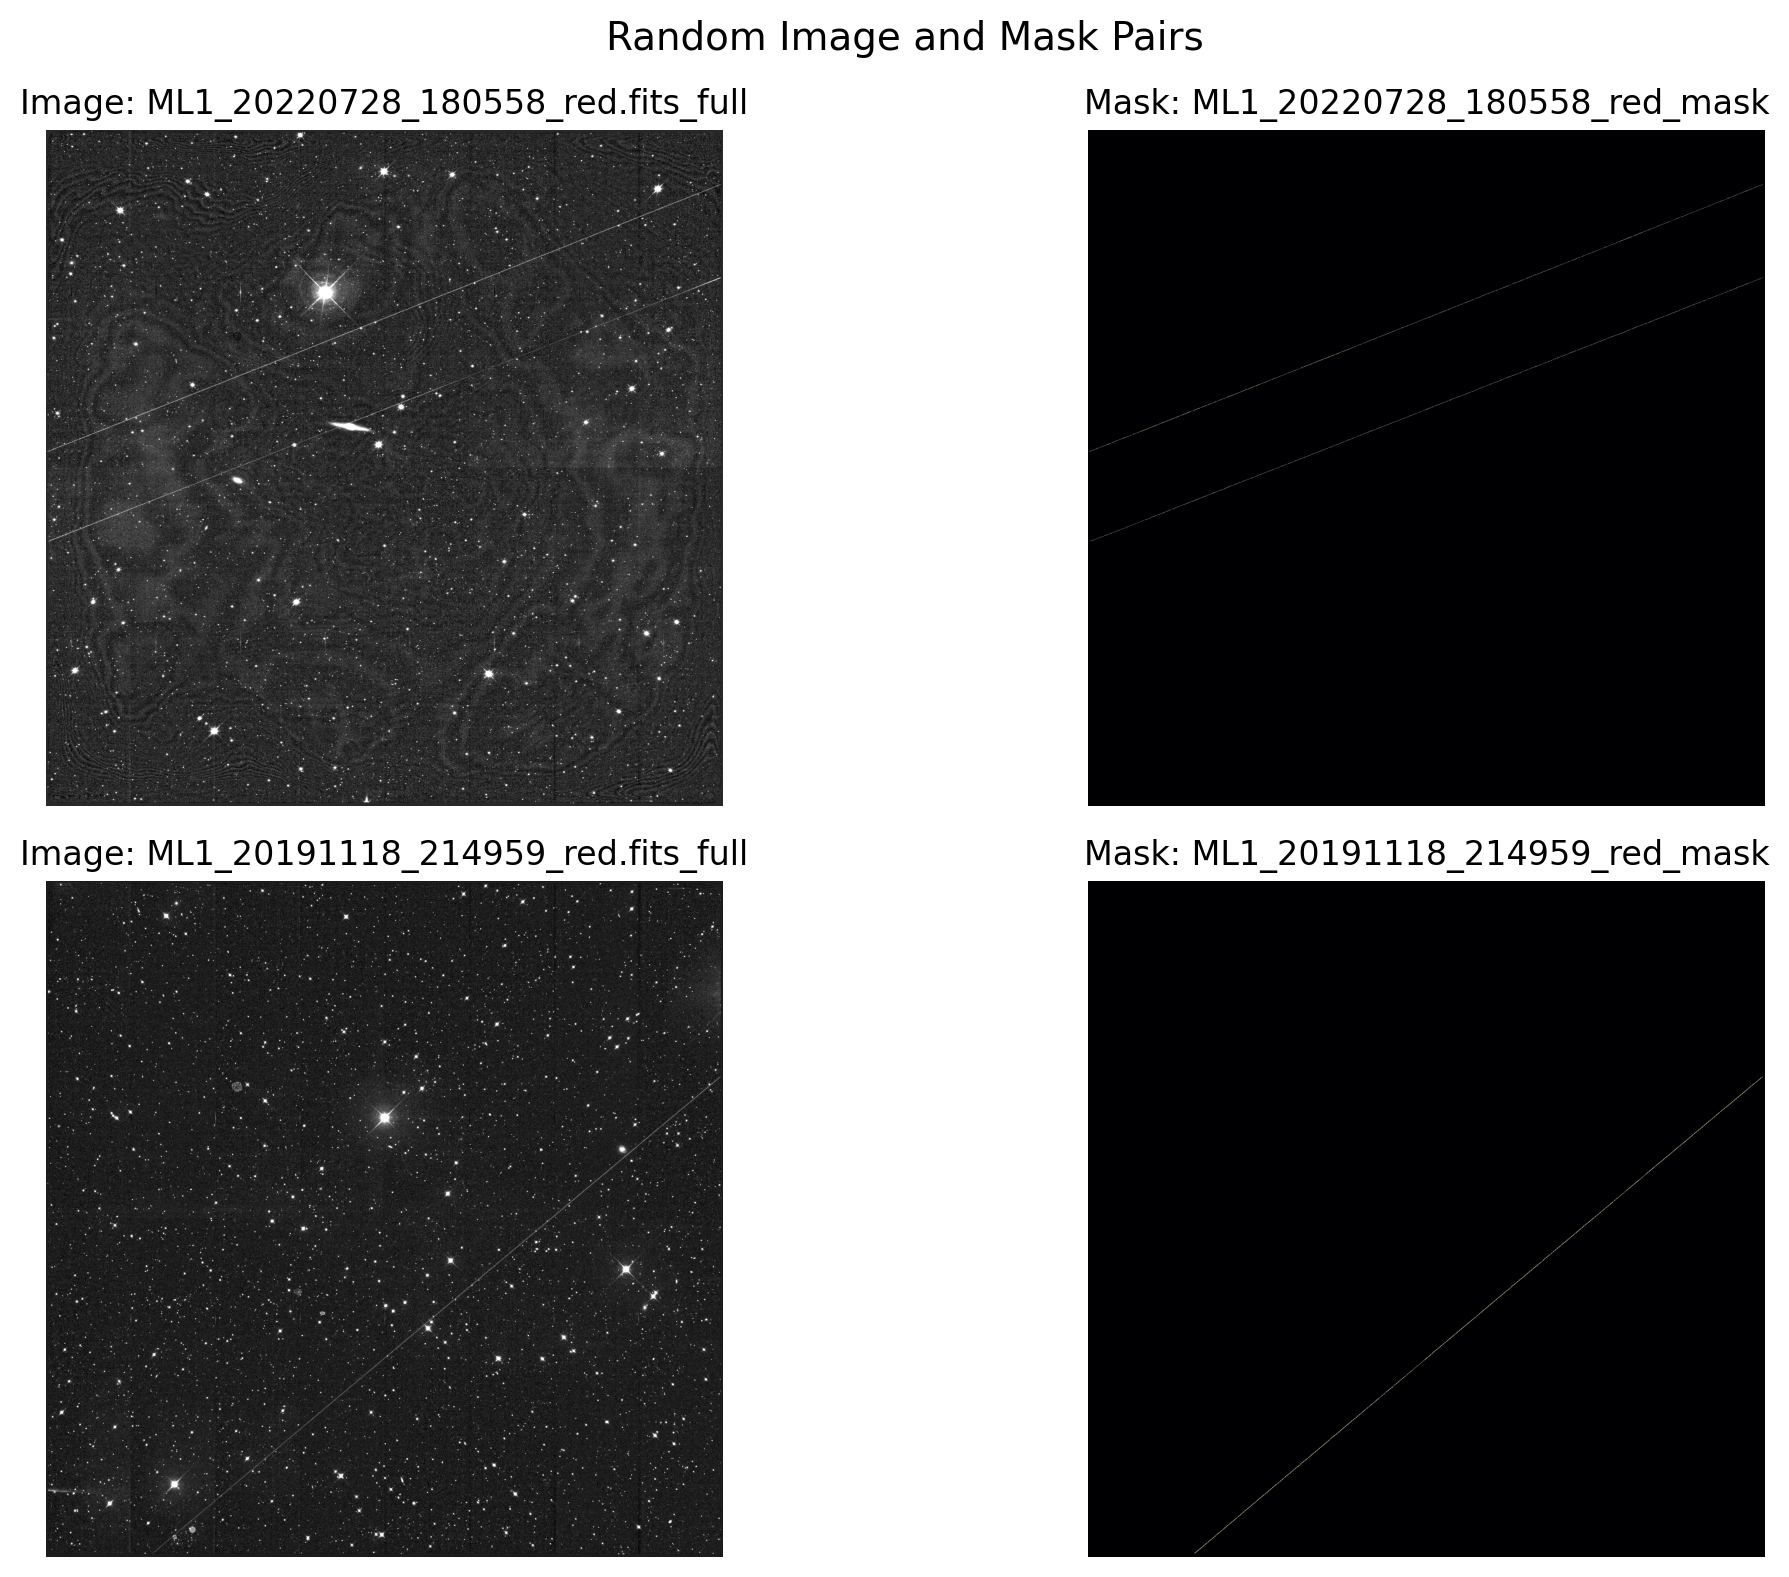
\includegraphics[width=0.92\linewidth]{../results/figures/eda_random_image_mask_pairs.png}
  \caption{Example image--mask pairs from the labelled subset: 8-bit PNG
           renders with hand-annotated binary trail masks. Trails are long,
           near-linear features against a crowded stellar background.}
  \label{fig:data_examples}
\end{figure}

\section{Exploratory analysis}
\label{sec:eda}

Exploratory analysis characterises the trail population and the number of
labelled trail pixels per image, which the splits must balance. Annotated trails
are long, near-linear features:
connected components have small minor-axis widths and high aspect ratios, and
many trails cross several adjacent patches. The per-image trail-pixel count is
heavily skewed, which motivates the stratified split of
Section~\ref{sec:splits} rather than a random split over images.
Filename-derived observation dates span 2017--2023, dominated by 2022
exposures; because exposures and observing conditions are not normalised, these
dates are purely descriptive.

\section{Patch extraction and class imbalance}
\label{sec:patching}

Full frames are too large for direct training. Patches are extracted at
$528\times528$ pixels with stride $528$, yielding exactly $400$ non-overlapping
patches per image ($20\times20$ grid). The natural patch distribution is highly
imbalanced, with approximately $93$--$94\,\%$ of full-grid patches containing
no trail pixels. To form the sampled patch manifests (patch lists used by the
training and evaluation code), all positive patches are retained and negatives
are down-sampled to a $1{:}3$ pos:neg ratio i.e., three
negative patches drawn for each positive patch. Figure~\ref{fig:data_flow}
gives the realised 528-pixel manifest sizes used by the final run.

The sampled test set is the main internal test population because it has the
same $1{:}3$ pos:neg prior as the validation set used for threshold
selection. A separate parity test set keeps every test-frame patch, including
all negatives, to restore the natural empty-patch prevalence for the
paper-facing precision check (Figure~\ref{fig:data_flow}); it is never used for
model or threshold selection. This separation is crucial because adding many empty
patches primarily changes precision: recall is computed over retained positive
patches, whereas the additional negatives can introduce false positives.

\section{Dataset splits}
\label{sec:splits}

Figure~\ref{fig:data_flow} summarises the path from frames to evaluation
manifests. Splits are performed at image level, never after patching, so
every patch from a given frame remains in the same split. The 178
images are stratified by total trail-pixel count into four quartile groups,
and the nominal $0.70/0.15/0.15$ ratios are applied within each group with
flooring; the remainder goes to test. The realised split is therefore
\textbf{122 train / 24 validation / 32 test} ($0.685/0.135/0.180$), quoted
throughout. This is leakage-safe and conservative, reserving a relatively large
held-out fraction for evaluation, with splits seeded ($2804$).

\begin{figure}[htbp]
  \centering
  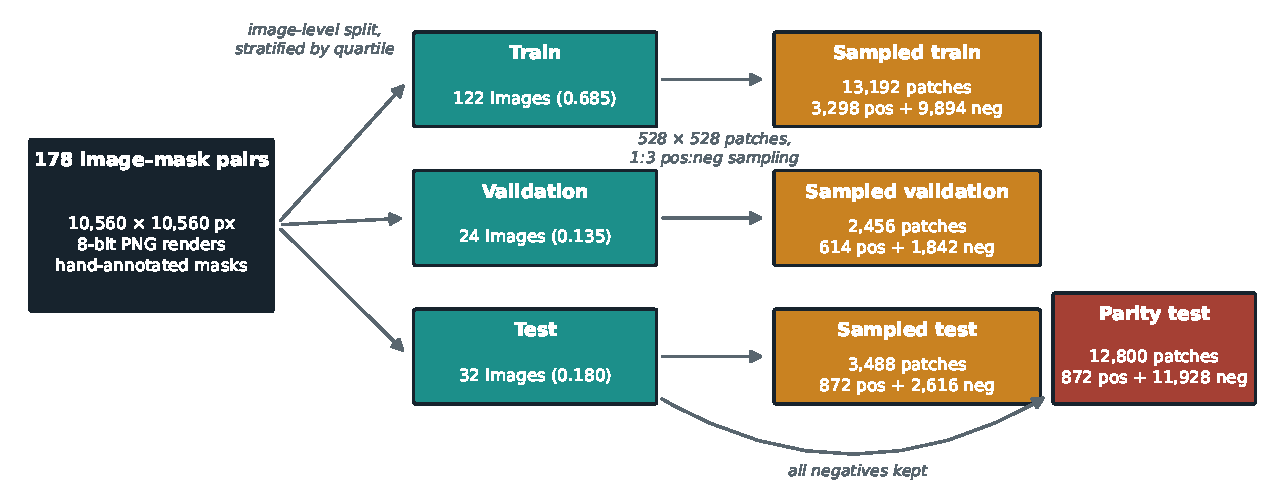
\includegraphics[width=0.92\linewidth]{../results/figures/data_split_schematic.pdf}
  \caption{Data flow from the 178 labelled frames to the evaluation manifests.
           Sampled manifests drive training, threshold selection, and internal
           evaluation; the parity manifest restores all negatives for the
           paper-facing precision check and is never used for selection.}
  \label{fig:data_flow}
\end{figure}

\section{Mask quality}
\label{sec:mask_quality}

Beyond visual inspection, connected-component measurements provide a simple
mask-quality check. Components have high aspect ratios and a median stroke width
near $6$\,px, estimated from distances to the nearest mask edge, confirming
genuinely linear structures; the densest patches adequately cover the visible
trails (Figure~\ref{fig:mask_quality}).

The masks are sufficient for supervised training, with one characterised caveat:
full-frame overlays show occasional mask under-coverage at faint endpoints and
low-contrast stretches. If the model detects a visible trail segment omitted
from the mask, those pixels are still counted as false positives, so strict
label-referenced precision is a conservative estimate where masks omit visible
trail pixels. Section~\ref{sec:ext_boundary} quantifies this boundary disagreement; interpretations
are phrased as `consistent with' boundary disagreement, not as proof of label error.

\begin{figure}[htbp]
  \centering
  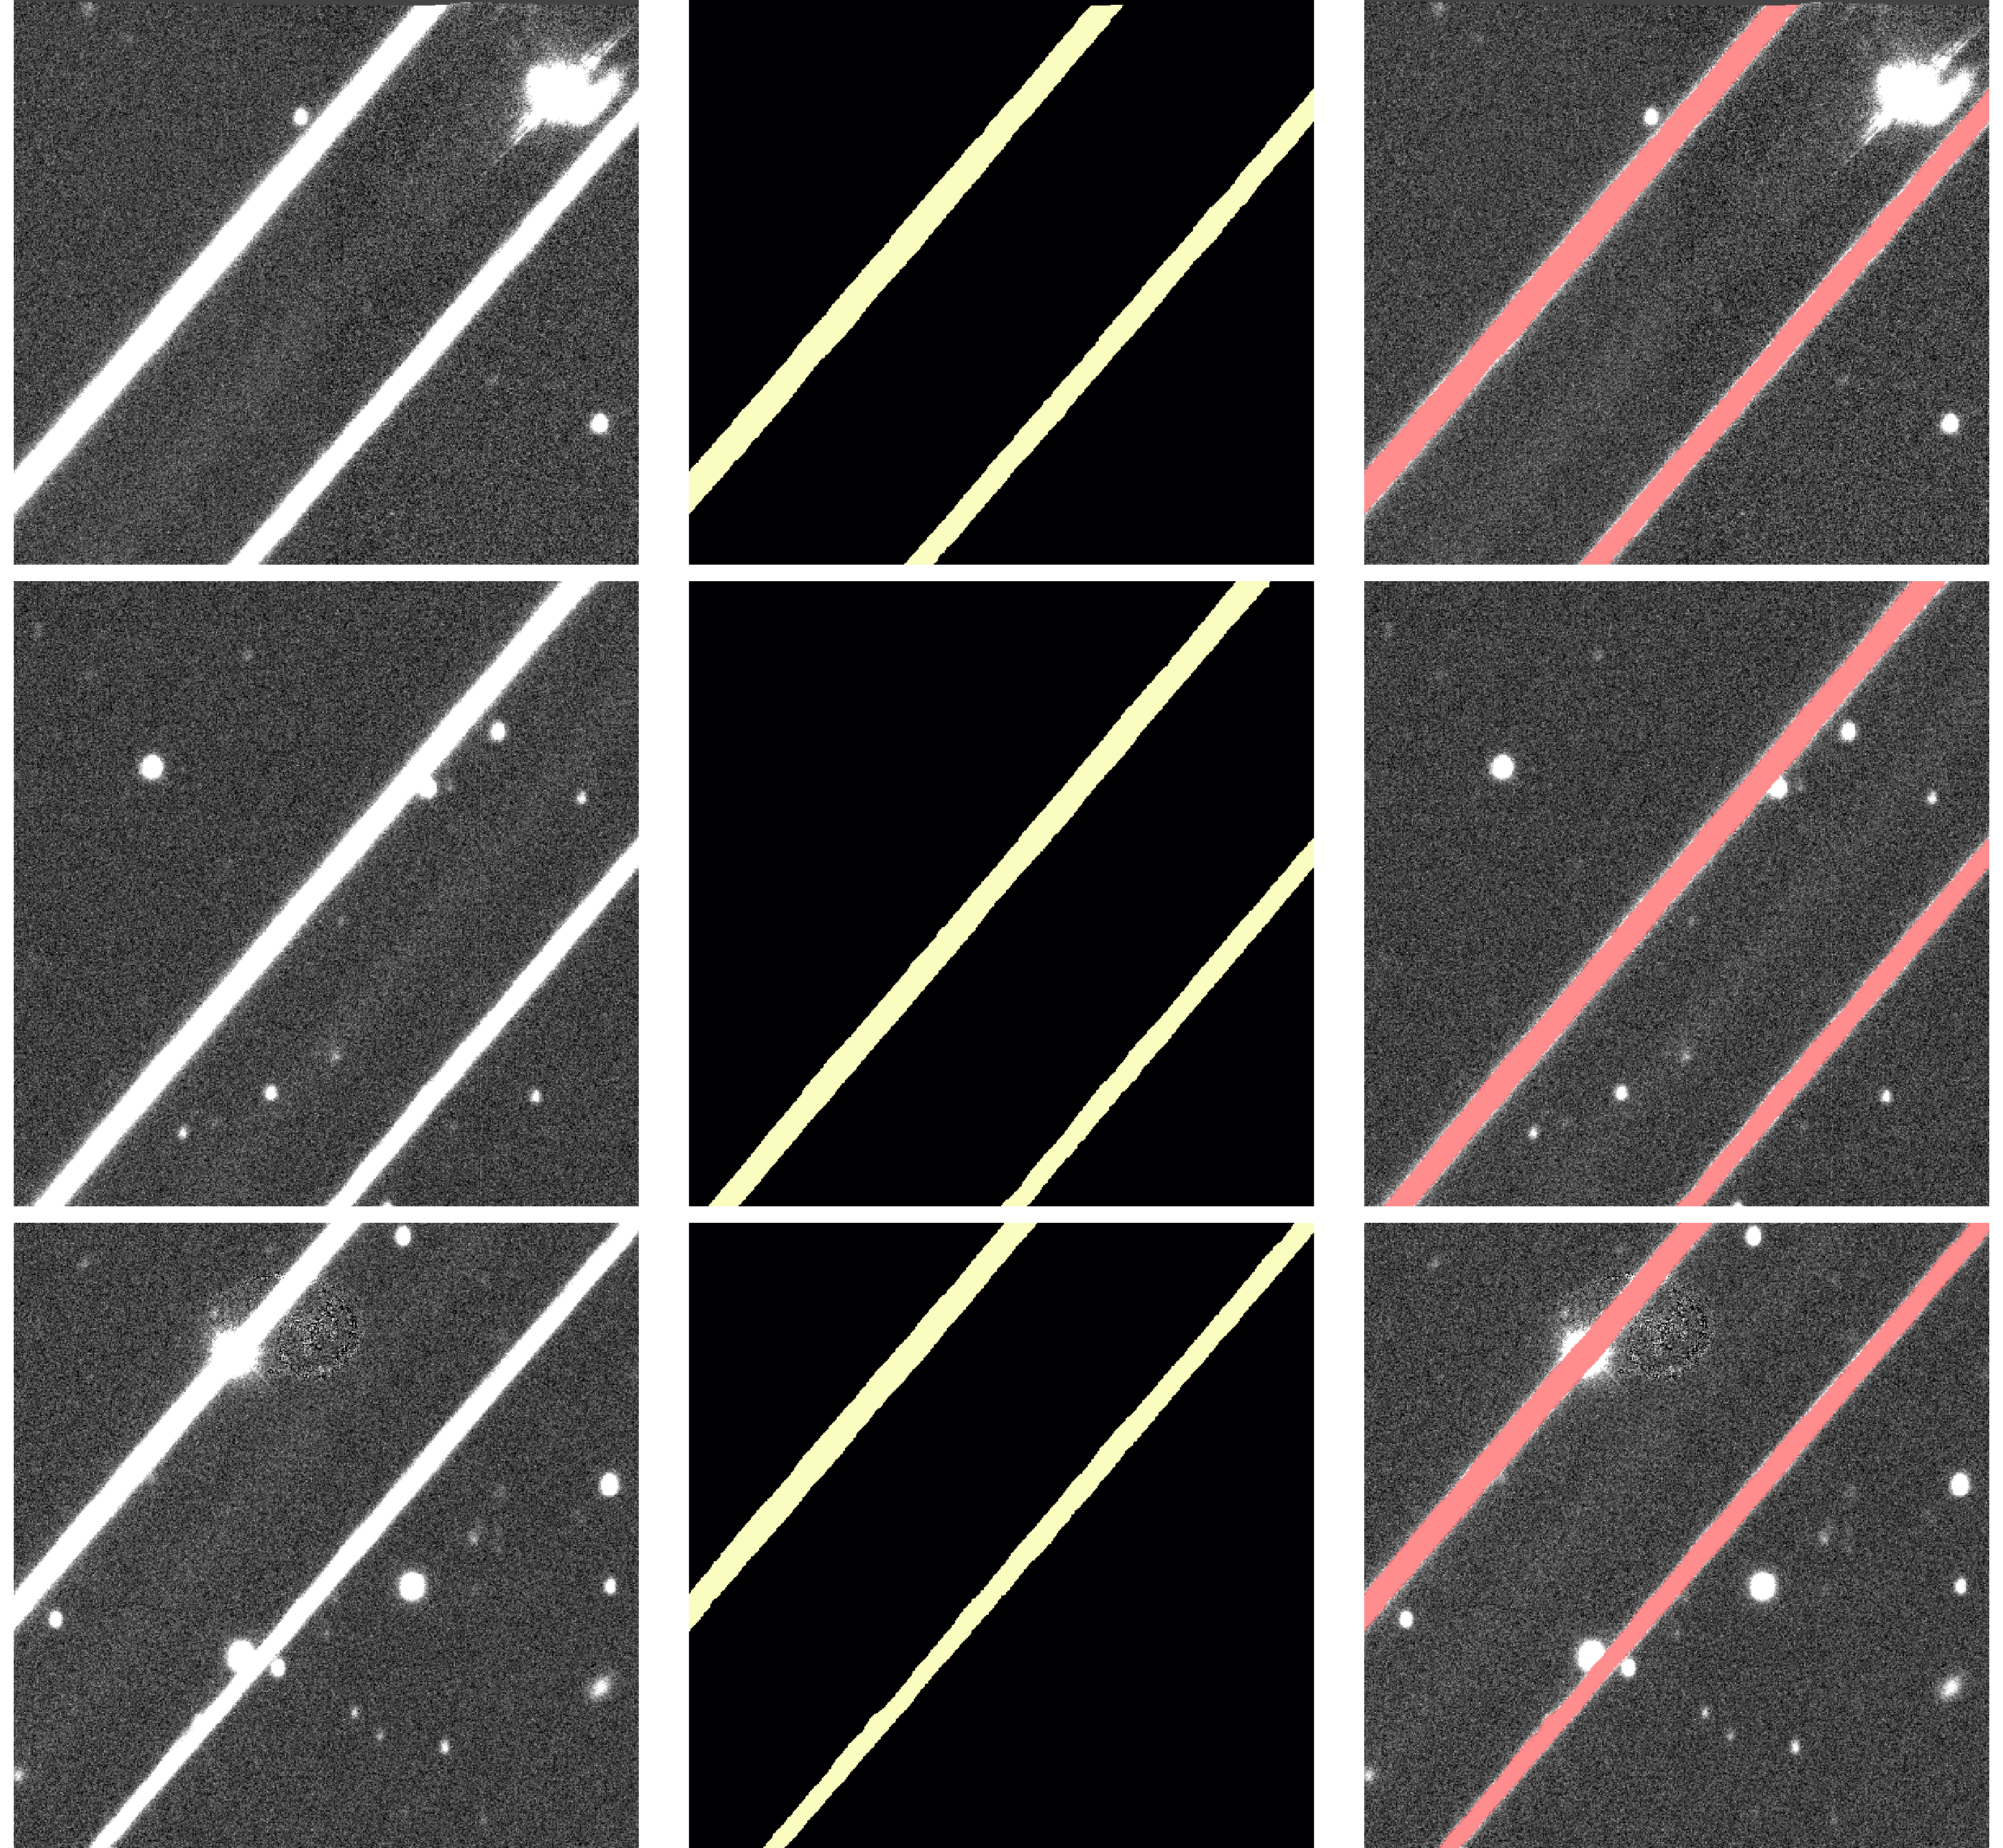
\includegraphics[width=0.92\linewidth]{../results/figures/eda_mask_inspection_grid_3row.png}
  \caption{Mask-quality inspection grid for three of the densest patches:
           image, annotated mask, and overlay (red). The masks track the
           visible trails; the residual concern is mask under-coverage at faint
           endpoints, quantified in Section~\ref{sec:ext_boundary}.}
  \label{fig:mask_quality}
\end{figure}

%%%%%%%%%%%%%%%%%%%%%%%%%%%%%%%%%%%%%%%%%%%%%%%%%%%%%%%%%%%%%%%%%%%%%%%%%%%%%%%%
%% CHAPTER 3 -- Methodology (why this method)
%% Scope: the rationale layer. Justify the approach -- learned segmentation plus
%% geometric post-processing, the U-Net choice, the loss family, image-level
%% splits and validation-only selection, and the evaluation philosophy. The
%% concrete configuration lives in Ch4.
%%%%%
\chapter{Methodology}
\label{ch:methodology}

\section{Problem formulation}
\label{sec:formulation}

Trail detection is posed as patch-wise binary pixel segmentation. Given a
$528\times528$ single-channel display-space patch, the model estimates a
per-pixel probability that each pixel belongs to a satellite trail rather than
background. Thus, the required output is a mask for downstream cleaning, not
a catalogue of satellite identities or trail instances.

This is semantic segmentation: pixels are labelled by class, not assigned to
individual trail instances. Crossing or near-parallel trails within a patch are
simply ``trail'', so pixel-level metrics
cannot distinguish merged from separated trails. The formulation is label-referenced:
success is measured against the available binary masks, so boundary placement
and mask under-coverage impact precision.

\section{Why learned segmentation with geometric post-processing}
\label{sec:why_method}

The pipeline pairs a learned segmentation stage with a classical geometric stage.
A U-Net produces a soft-detection map that preserves weak, spatially extended
evidence of a faint trail. A classical Hough detector applied directly to the
raw image responds mainly to stars, galaxies, and diffraction
structure. In a validation-tuned raw-image Hough implementation, precision was
only about $10^{-3}$, confirming that raw-image Hough voting is an insufficient
masking baseline. Thus, the probabilistic Hough transform is used after the
U-Net, where the input is already a trail-probability canvas rather than a
crowded sky image. There, it can
exploit the prior that a trail is globally linear to bridge gaps and recover
continuous trail structure. The remaining methodological
choices follow this framing: the U-Net supplies pixel-level segmentation, the
BCE--Dice loss handles severe foreground imbalance, and evaluation protocols
separate selection, prevalence, and label-boundary effects.

\section{Why a U-Net}
\label{sec:why_unet}

The U-Net encoder--decoder with skip connections \citep{ronneberger2015} preserves full spatial
resolution. This is essential for thin, elongated, sparse targets, while its
encoder path still supplies enough context to distinguish trails from stellar
structure and background gradients. The same architecture underpins close
astronomical artefact detectors such as deepCR \citep{zhang2020} and MaxiMask
\citep{paillassa2020}, supporting its suitability here.

More elaborate variants are treated as follow-up tests rather than replacements
for the replication baseline; Section~\ref{sec:ext_attention} tests whether
adding attention gates changes the residual error pattern. Transformer-style
segmenters, such as ViT, are not explored as replication baselines because they
would change the detector family and introduce data and tuning demands that are
poorly matched to this relatively small dataset.

\section{Why a combined BCE and Dice loss}
\label{sec:why_loss}

The foreground occupies a tiny fraction of pixels, so a pure cross-entropy
objective is dominated by easy background. The Dice term measures region overlap
and is less dominated by the background majority \citep{milletari2016}.
Combining it with binary cross-entropy keeps per-pixel calibration while
following the Combo-loss pattern for severely imbalanced segmentation
\citep{taghanaki2019}. Binary cross-entropy also allows a positive-class weight,
\texttt{pos\_weight}, to penalise missed trail pixels further. However, this was not
applied in the final pipeline as the $1{:}3$ patch sampling
and Dice term already address the imbalance. Stacking another class weight would
bias the model towards over-prediction.

\section{Evaluation philosophy}
\label{sec:eval_philosophy}

Four principles govern the evaluation. Model and threshold selection are
pre-registered and validation-only, so no test metric is inspected before the
configuration is locked. Sampled and all-negative test metrics are kept distinct:
the sampled set matches the validation prior, while the all-negative set restores
the natural empty-patch prevalence used for the paper-facing comparison. Uncertainty
treats the source image, not the patch, as the independent unit, because patches
from one frame share background, atmospheric image quality, and annotation
structure. Finally,
because masks omit some visible trail pixels (Section~\ref{sec:mask_quality}),
strict pixel-overlap scores are complemented by topology-aware (clDice),
false-positive distance, and boundary-tolerant metrics
(Section~\ref{sec:metrics}).

%%%%%%%%%%%%%%%%%%%%%%%%%%%%%%%%%%%%%%%%%%%%%%%%%%%%%%%%%%%%%%%%%%%%%%%%%%%%%%%%
%% CHAPTER 4 -- Training, architecture, and data pipeline
%% Scope: the concrete, settled configuration. Most of this chapter is
%% methodology boilerplate that will not change and is filled in below.
%%%%%
\chapter{Training, Architecture, and Data Pipeline}
\label{ch:pipeline}

\section{Data pipeline}
\label{sec:datapipeline}

The on-disk patch builder extracts $528\times528$ patches at stride $528$
(Section~\ref{sec:patching}), writing canonical orientations at the $1{:}3$
sampling ratio. The builder records
the source image, split, patch coordinates, positive-pixel fraction, and
full-image display-space mean and standard deviation in the manifest. The last
two fields implement the \texttt{full\_image} normalisation mode: each
patch is converted to $[0,1]$ and normalised with the statistics of its parent
image, matching the paper's per-image standardisation better than a
per-patch z-score.

\subsection{Data augmentation}
\label{sec:augmentation}

Training patches receive random horizontal flips, vertical flips, and
$k\times90^{\circ}$ rotations applied identically to image and mask at load
time, so stored patches keep their canonical orientation and can appear in
different orientations across epochs; validation and test patches are not
geometrically augmented. Training images also receive signal-dependent
stochastic noise (images only, never masks or evaluation splits). For a
patch-pixel value $p\in[0,1]$ the augmentation samples
\[
  p_{\mathrm{noisy}} =
  \mathrm{clip}\!\left(p + \mathcal{N}\!\left(0,\;
  m\sqrt{\alpha p + \beta^{2}}\right),\,0,\,1\right),
\]
where $m$ is the noise multiplier and $\alpha,\beta$ are calibrated once from
empty-mask training patches by
\texttt{scripts/data/compute\_background\_noise\_stats.py}, so the injected
noise matches the measured background variation. The locked calibration uses
$9{,}894$ empty train patches, giving $\alpha=0.0209$ and $\beta=0.0886$.
It is described as
signal-dependent stochastic noise rather than Poisson--Gaussian CCD noise
because the inputs are display renders, not calibrated electron counts. The
active configuration fixes $m=1.0$ as a calibrated,
robustness-motivated choice rather than a tuned gain; a preliminary three-seed
screen over multipliers $\{0.5, 1.0, 2.0\}$ found no gain meeting the
preregistered adoption criterion.

\section{Network architecture}
\label{sec:architecture}

\begin{figure}[htbp]
  \centering
  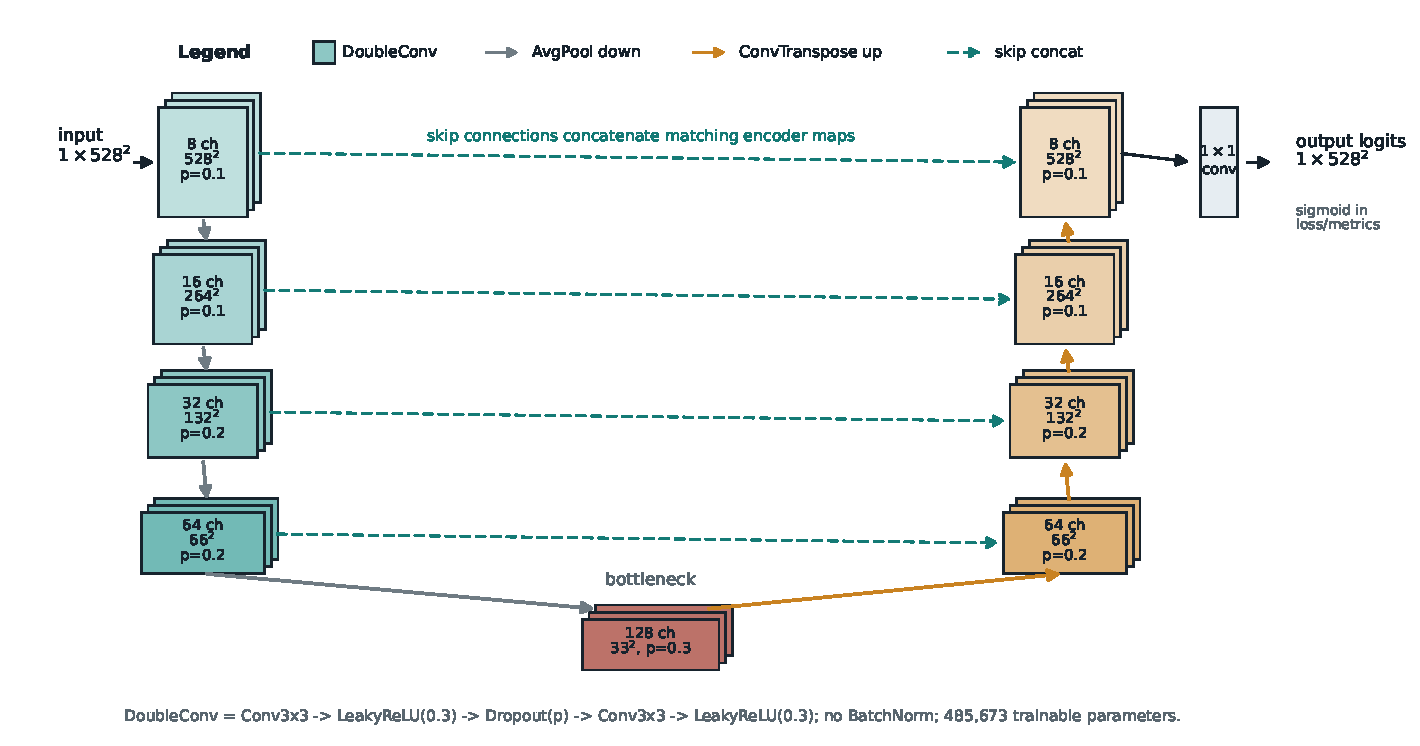
\includegraphics[width=0.92\linewidth]{../results/figures/unet_architecture.pdf}
  \caption{Architecture-faithful U-Net. Encoder widths $8\to16\to32\to64$ with a
           $128$-channel bottleneck, average-pooling downsampling,
           transposed-convolution upsampling, and skip concatenation at each
           level. Each block is two $3\times3$ convolutions with \mbox{LeakyReLU(0.3)}
           and in-block dropout.}
  \label{fig:unet}
\end{figure}

The replication network (Figure~\ref{fig:unet}) follows the released Stoppa
et al.\ model configuration rather than only the paper's textual description: an
encoder--decoder with skip
connections and filters progressing $8\to16\to32\to64\to128$, average-pooling
downsampling, transposed-convolution upsampling, and LeakyReLU activations with
slope $0.3$. Each double-convolution block follows
\texttt{Conv2d $\to$ LeakyReLU $\to$ Dropout $\to$ Conv2d $\to$ LeakyReLU}, with
element-wise dropout in all nine blocks. The dropout rates from stem to final
decoder block are
\[
  0.1,\ 0.1,\ 0.2,\ 0.2,\ 0.3,\ 0.2,\ 0.2,\ 0.1,\ 0.1 .
\]
The network uses no batch normalisation. The $3\times3$ convolutions use He-normal initialisation
\citep{he2015delving}; the transposed convolutions and the final $1\times1$ head use
Glorot-uniform initialisation; all biases are initialised to zero. Inputs are
$528\times528$ single-channel patches and the output is a single-channel logit
map of identical spatial dimensions: the model returns logits, and the sigmoid
is applied explicitly in the loss, threshold, Hough, and visualisation paths.
The network has $485{,}673$ trainable parameters
(\texttt{base\_channels}~$=8$).

\section{Loss function}
\label{sec:loss}

Training uses a combined binary cross-entropy (BCE) and squared-Dice loss:
\begin{equation}
  \mathcal{L} = \lambda_{\mathrm{BCE}}\,\mathcal{L}_{\mathrm{BCE}}
              + \lambda_{\mathrm{Dice}}\,\mathcal{L}_{\mathrm{Dice}},
  \qquad \lambda_{\mathrm{Dice}} = 1 - \lambda_{\mathrm{BCE}},
\end{equation}
where
\[
  \mathcal{L}_{\mathrm{Dice}}
  = 1 - \frac{2\sum_i p_i g_i + \epsilon}
             {\sum_i p_i^{2} + \sum_i g_i^{2} + \epsilon},
  \qquad \epsilon = 10^{-4},
\]
with $p_i$ the sigmoid probabilities and $g_i$ the binary targets. The Dice term
follows \citet{milletari2016}; combined with BCE it sits in the Combo-loss
family of \citet{taghanaki2019}. The BCE term uses
\texttt{BCEWithLogitsLoss} without a class-balancing \texttt{pos\_weight},
matching the paper-faithful path and avoiding a second imbalance correction on
top of the sampled patch prior. Losses are evaluated in FP32 even when the
forward pass uses BF16 autocast \citep{micikevicius2018,kalamkar2019}.

\section{Hyperparameter search}
\label{sec:optuna}

Hyperparameter search uses Optuna \citep{akiba2019} with a tree-structured
Parzen estimator and median pruner ($n_{\mathrm{startup}}=15$, 10 warm-up
epochs). Forty-five trials are balanced across batch sizes $\{8,16,32\}$
(fifteen each) after a preliminary free-sampling sweep concentrated most of its
trials on one batch size and pruned large-batch trials under a higher
conditional learning-rate ceiling. The searched continuous hyperparameters are
learning rate (log-uniform in $[10^{-4},10^{-3}]$) and BCE weight
$\lambda_{\mathrm{BCE}}$ (uniform in $[0.2,0.8]$); dropout, normalisation, and
noise multiplier are fixed. Each trial runs for 20 epochs and is scored by
threshold-swept validation $F_1$, matching the final selection criterion.
Pruning uses in-epoch validation Dice at the fixed training threshold as an
efficiency heuristic, while only completed trials are rescored by swept
validation $F_1$. The top five trials by validation $F_1$ are retrained for 75
epochs at five seeds
($2804, 1234, 42, 7, 13$), and the winner is chosen by mean threshold-swept
validation $F_1$ across seeds \emph{before any test metric is inspected}. The
preregistered tie-breaker, applied when trial means fall within $0.001$
validation $F_1$, prefers lower batch size, then lower learning rate, then lower
trial index. The selected base U-Net is trial~44
(\texttt{batch\_size}=32, learning rate $2.89\times10^{-4}$,
$\lambda_{\mathrm{BCE}}=0.655$), with mean validation $F_1=0.854$ across the
five retrained seeds; trial~32 reached a marginally higher raw mean ($0.855$),
but trial~44 won the within-$0.001$ tie band on the lower-learning-rate rule.
The full search space is given in Appendix~\ref{app:hparam}.

\section{Threshold selection}
\label{sec:threshold}

A precision--recall curve is swept on the validation set to select the
$F_1$-optimal threshold, which is applied unchanged to the test evaluation;
each reported seed uses its own validation-selected threshold, with $0.45$ for
the canonical seed 2804 (the paper fixes $0.58$). Within each run, the saved
best epoch is selected by validation Dice at the fixed training threshold, and
the saved checkpoint is then threshold-swept for trial ranking and
operating-point selection; checkpointing and operating-point selection
therefore use related, but different, validation criteria.

\section{Hough post-processing}
\label{sec:hough}

A probabilistic Hough transform \citep{matas2000} (\texttt{cv2.HoughLinesP}) is
applied to a lower-threshold probability canvas to recover faint, linear
detections below the segmentation threshold.
For each test image the per-patch sigmoid probability maps are max-pooled into
a canvas before Hough voting. The sampled evaluation uses the $1{:}3$ patch
support, while the parity Hough comparison uses full $528$\,px tiling over every
test image; an independent full-coverage tiled pass reproduced that
parity canvas pixel-for-pixel, ruling out a patch-sampling or seam gap. The
canvas is thresholded at $t_{\mathrm{Hough}}=0.1$,
after which \texttt{HoughLinesP} is run with a vote threshold of $50$, a minimum
line length of $100$\,px, and a maximum gap of $250$\,px, matching the released
ASTA reference implementation of \citet{stoppa2024}. Detected segments are drawn
back onto the canvas at $3$\,px thickness, making line-rasterisation convention
the main remaining comparability caveat for strict precision.

\section{Patch CNN classifier for the two-stage variant}
\label{sec:classifier}

The two-stage variant of Section~\ref{sec:ext_twostage} places a lightweight
convolutional neural network (CNN) patch classifier in front of the U-Net. The
classifier is intentionally simple: a four-block strided encoder followed by
global average pooling and a single fully connected logit head, trained on the
sampled training manifest with labels derived from the patch positive-pixel fraction and a
\texttt{pos\_weight} equal to the train-split negative-to-positive ratio.
Validation reports both the maximum-$F_1$ and a high-recall
(recall~$\ge0.99$) operating point, because a patch rejected by the gate is
unrecoverable downstream. The classifier and the U-Net are trained
independently and composed only at inference, keeping the gate a
single-variable change to the locked pipeline; the classifier never sees test
data during U-Net selection.

\section{Evaluation metrics}
\label{sec:metrics}

Segmentation quality is reported with pixel precision, recall, Dice (equal to
$F_1$ for binary masks), and IoU. Topology is assessed with the centreline Dice
(clDice) \citep{shit2021}. Boundary disagreement is isolated with a
boundary-tolerant precision/recall/$F_1$ score at
$k\in\{0,1,2,3\}$\,px, where $k=0$ is the strict metric and $k>0$ allows a
predicted pixel and a ground-truth pixel to match within a small spatial
tolerance. The spatial structure of false positives is summarised by their
distance to the nearest ground-truth trail pixel, with whole-patch false
positives reported separately because they have no defined trail distance.
Uncertainty is quantified primarily by a cluster bootstrap over source images,
resampling images with replacement and aggregating their patches before
recomputing each metric; a patch-level bootstrap is reported only as a
secondary diagnostic.

\section{Determinism and reproducibility}
\label{sec:reproducibility}

All experiments seed the Python, NumPy, and PyTorch generators (canonical seed
$2804$), enable cuDNN deterministic mode, fix the cuBLAS workspace, and seed
DataLoader workers. Residual GPU non-determinism is absorbed by five-seed
retraining of the top trials and seed-averaged reporting. The probabilistic
Hough stage (\texttt{cv2.HoughLinesP}) is the one post-hoc step whose OpenCV
RNG is not separately seeded, so its reruns are near- but not bit-identical.

\section{Software engineering}
\label{sec:software}

The code is packaged as an installable Python project with module-level command-line interfaces for
each pipeline stage. Experiments use YAML configuration plus runtime overrides,
so runs are reproducible from configuration and seed.

Correctness is checked by a \texttt{pytest} suite covering image and mask
pairing, patch geometry, the recovered architecture, loss and segmentation
metrics, the shared Hough runner, and training entry points; Ruff handles static
checks. Separate CUDA and CPU requirement files are maintained, and a portable
CPU Docker image runs the tests by default. NumPy-style docstrings are rendered
with Sphinx and served on ReadTheDocs; routines are referenced by file, for
example \texttt{src/training/train\_unet.py}.

%%%%%%%%%%%%%%%%%%%%%%%%%%%%%%%%%%%%%%%%%%%%%%%%%%%%%%%%%%%%%%%%%%%%%%%%%%%%%%%%
%% CHAPTER 5 -- Analysis and comparison
%% Scope: replication vs the paper, then the precision-gap diagnosis and the
%% model/training/inference sensitivity tests that support it.
%%%%%
\chapter{Replication and Error Diagnosis}
\label{ch:analysis}

\section{Replication of the ASTA detector}
\label{sec:replication}

The validation-selected winner (trial~44; Section~\ref{sec:selection}) is
evaluated on the held-out test images at its selected threshold of
$0.45$. On the sampled test set ($1{:}3$ positive:negative) the single-seed model
reaches precision $0.852$, recall $0.918$, and Dice $0.884$, with a five-seed mean
of precision $0.847$ and recall $0.923$ (Table~\ref{tab:replication},
Figure~\ref{fig:replication}). On the parity test set, precision falls to
$0.780$ at unchanged recall ($0.918$), as expected once the negative base rate
is restored. Recall is therefore reproduced at close
to the paper's level, while strict precision sits below the paper's $0.94$. The
rest of the chapter analyses where that gap comes from, not
treating it as an optimisation target.

\begin{table}[htbp]
  \centering
  \caption{Replication comparison against Stoppa et al.\ (2024). Paper metrics
           are at threshold $0.58$ on a 20{,}000-patch test set; this work uses
           the realised $122/24/32$ image split and the validation-selected
           threshold $0.45$ (per-seed $0.41$--$0.50$). Cluster-bootstrap intervals are in
           Section~\ref{sec:bootstrap}. Dashes mean that exact values are not
           numerically tabulated in the paper.}
  \label{tab:replication}
  \small
  \begin{tabular}{p{0.40\textwidth}ccccc}
    \toprule
    Run & Threshold & Precision & Recall & Dice & IoU \\
    \midrule
    Stoppa et al.\ (2024)              & 0.58 & 0.94  & 0.94  & ---   & ---   \\
    \midrule
    This work, sampled (single seed)   & 0.45 & 0.852 & 0.918 & 0.884 & 0.791 \\
    This work, sampled (5-seed mean)   & $0.41$--$0.50$ & 0.847 & 0.923 & 0.884 & 0.792 \\
    This work, parity (single seed)    & 0.45 & 0.780 & 0.918 & 0.843 & 0.729 \\
    \bottomrule
  \end{tabular}
\end{table}

\begin{figure}[htbp]
  \centering
  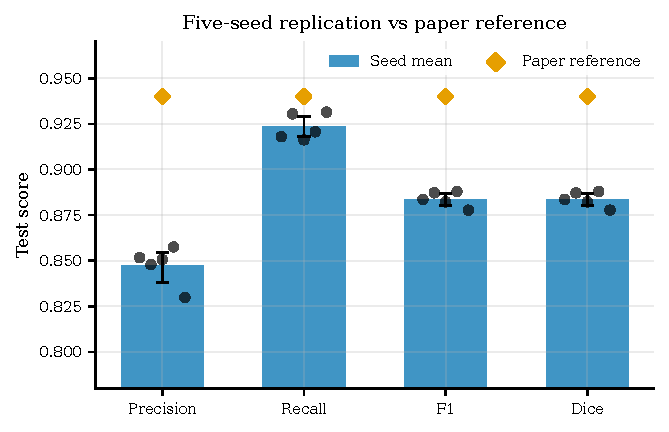
\includegraphics[width=0.85\textwidth]{../results/figures/thesis_1_multiseed_replication.pdf}
  \caption{Five-seed replication summary for the locked validation-selected
           U-Net configuration. Paper-reference markers are shown only for the
           explicitly reported precision and recall values.}
  \label{fig:replication}
\end{figure}

\section{Validation-locked model selection}
\label{sec:selection}

Trial~44 was selected by mean validation $F_1$ across the five-seed retraining
of the top five trials, before any test metric was inspected
(Section~\ref{sec:optuna}; Figure~\ref{fig:sweep_selection}). Its validation
precision--recall sweep sets the operating threshold of $0.45$, carried
unchanged into the canonical seed-2804 test evaluation. Across the five reported seeds,
the validation-selected thresholds range from $0.41$ to $0.50$, and each seed is
evaluated at its own validation-selected threshold. Figure~\ref{fig:pr_curve}
shows the validation sweep for the canonical seed; the $F_1$ plateau is flat
between roughly $0.4$ and $0.6$, so the operating point is not
finely tuned.

\begin{figure}[htbp]
  \centering
  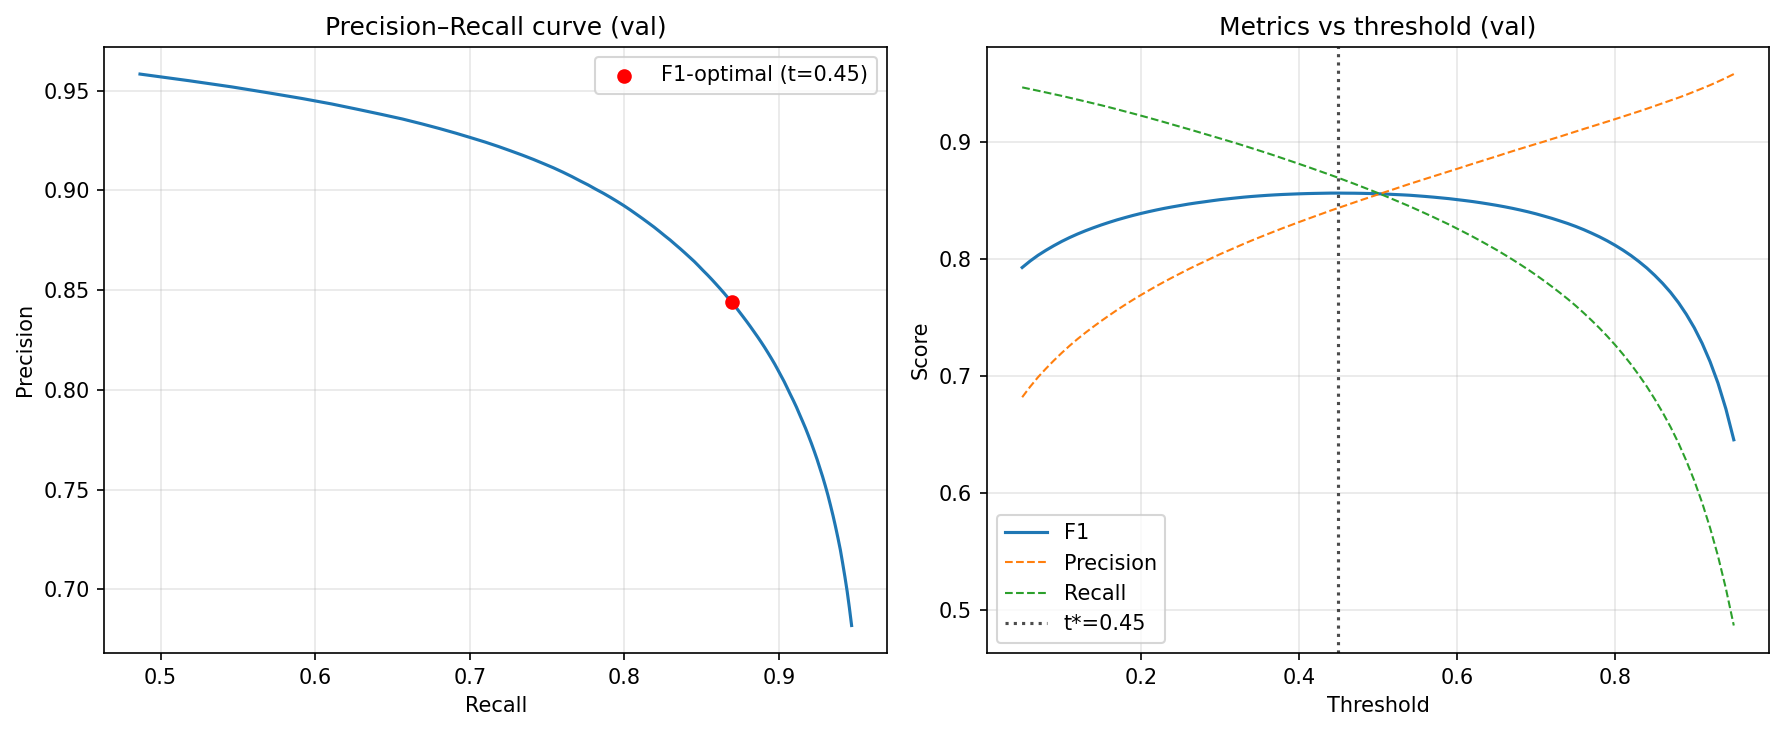
\includegraphics[width=0.92\linewidth]{../results/figures/threshold_sweep_winner_t44_s2804_pr_curve.png}
  \caption{Validation sweep for the canonical seed-2804 winner: PR curve with
           the $F_1$-optimal point ($t^{*}=0.45$, left) and metrics versus
           threshold (right); the flat $F_1$ plateau spans the paper's fixed
           $0.58$.}
  \label{fig:pr_curve}
\end{figure}

\begin{figure}[htbp]
  \centering
  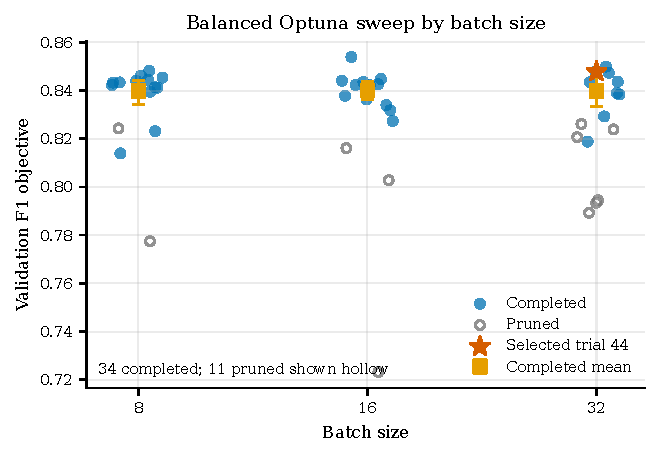
\includegraphics[width=0.85\textwidth]{../results/figures/thesis_7_sweep_selection.pdf}
  \caption{Balanced Optuna sweep and validation-only winner selection; pruned
           trials are hollow markers and the selected trial 44 is starred.}
  \label{fig:sweep_selection}
\end{figure}

\section{Hough improves pixel completeness}
\label{sec:hough_results}

Probabilistic Hough post-processing raises trail-pixel recall from $0.918$ to
$0.990$ for the canonical seed on the full-coverage parity canvas, equivalently
reducing the pixel-level false-negative rate from $0.082$ to $0.0105$
(five-seed mean $0.077\rightarrow0.0098$). This pixel-completeness rate is the
quantity comparable to the paper's reported $6.98\,\%\rightarrow3.38\,\%$, and
the independent full-coverage tiled check shows it is not a patch-sampling or seam
artefact. The image-level detection false-negative rate is degenerate here:
every positive test image is already hit by at least one predicted pixel, so it
is $0$ before and after Hough and is not comparable to the paper. At patch level,
the rate falls only from $0.122$ to $0.103$, since this stricter diagnostic
counts trail-bearing patches with no recovered pixel. This is why Hough is
treated here as a completeness mechanism, not a precision fix.

A qualitative post-hoc example (Figure~\ref{fig:hough_gap}) shows the
mechanism: the U-Net misses a trail stretch over a bright star, and Hough
recovers ground-truth pixels that appear only after the geometric stage. The
example is a mechanism illustration, not a benchmarked bridge-rate estimate.

\begin{figure}[htbp]
  \centering
  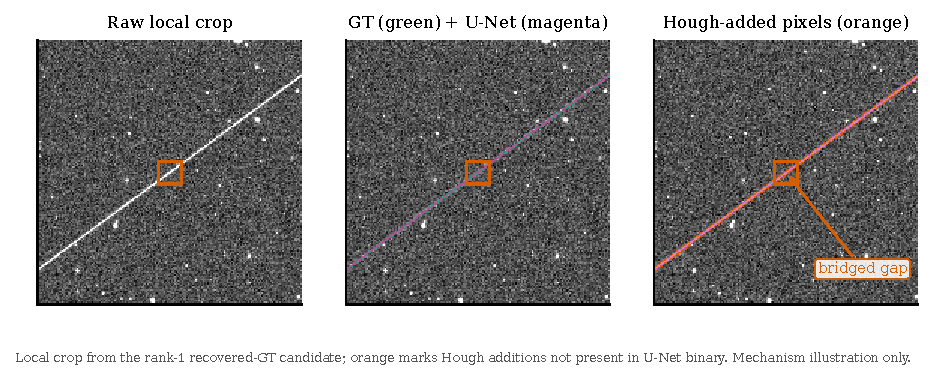
\includegraphics[width=0.9\textwidth]{../results/figures/hough_gap_bridge_example.pdf}
  \caption{Hough bridging a U-Net gap. Panels: raw image; ground truth (green)
           with U-Net prediction (magenta); U-Net (magenta) with Hough bridge
           (orange). Ground-truth pixels over the bright star are recovered
           only by Hough.}
  \label{fig:hough_gap}
\end{figure}

\section{Uncertainty quantification}
\label{sec:bootstrap}

Cluster-bootstrap $95\,\%$ intervals over the 32 test images ($1{,}000$
resamples, single-seed winner) are precision $0.852\,[0.806,\,0.891]$, recall
$0.918\,[0.888,\,0.946]$, Dice $0.884\,[0.857,\,0.904]$, and IoU
$0.791\,[0.749,\,0.825]$. These image-level intervals are several times wider
than the patch-level bootstrap (Dice $[0.876,\,0.892]$), which is reported only
as a secondary diagnostic; the 32 source images are the independent units. The
headline interval is therefore the image-cluster interval; the patch bootstrap is
included only to show how much patch-level resampling would understate
uncertainty. Across the five trial-44 seeds, the sampled-test means and sample
standard deviations are precision $0.847\pm0.010$, recall $0.923\pm0.007$, and
Dice $0.884\pm0.004$, so seed variation is smaller than the image-cluster
uncertainty but still visible.

\section{Qualitative prediction checks}
\label{sec:predictions}

\begin{figure}[htbp]
  \centering
  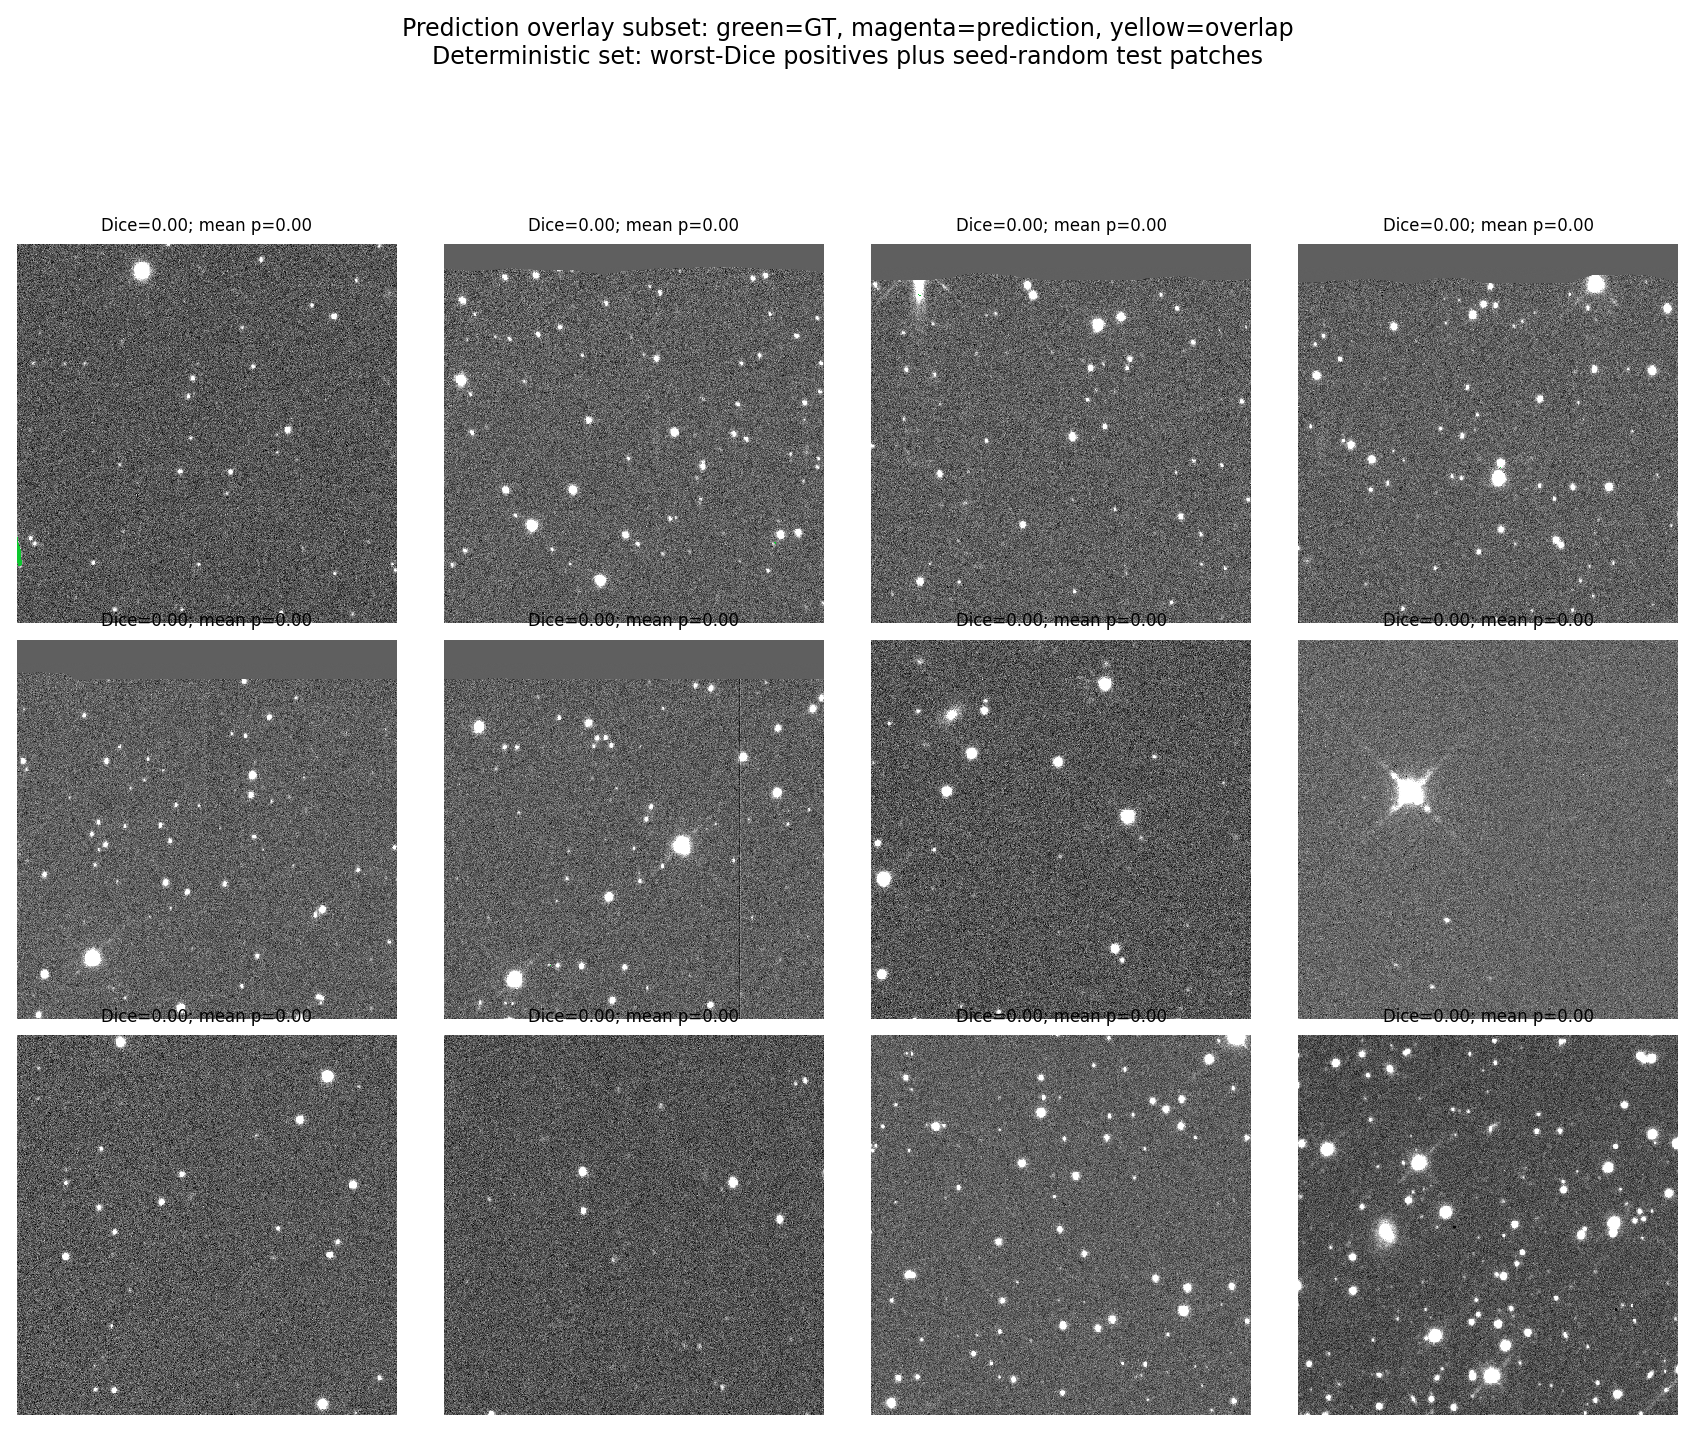
\includegraphics[width=0.92\linewidth]{../results/figures/predictions/overlay_grid_winner_t44_s2804.png}
  \caption{Diagnostic selection of test-patch predictions for the locked winner:
           image, ground-truth mask (green), and predicted mask (magenta), with
           overlap shown as magenta inside the green band.}
  \label{fig:predictions}
\end{figure}

A diagnostic selection of locked-winner test predictions is shown in
Figure~\ref{fig:predictions}; false-positive galleries for the winning U-Net and
attention variant on the same eight patches are in
Appendix~\ref{app:supplementary}. They include diffraction-spike examples:
low-Dice false positives on stellar structure and high-Dice cases where bright
stars are correctly ignored.

As a final qualitative check, the locked model was applied cold to nine
predeclared DECam frames with RECA-measured streaks
(Figure~\ref{fig:decam_cold_montage}). With no masks, no metric is reported; on
manual visual review, eight of nine visible streaks are fully traced, while the very
faint full-frame SORCE streak is traced along only about a tenth of its length
and counted as a miss. This sits at the low-contrast end predicted by
Section~\ref{sec:ext_faint}, illustrating out-of-domain behaviour rather than a
cross-dataset benchmark.

\begin{figure}[htbp]
  \centering
  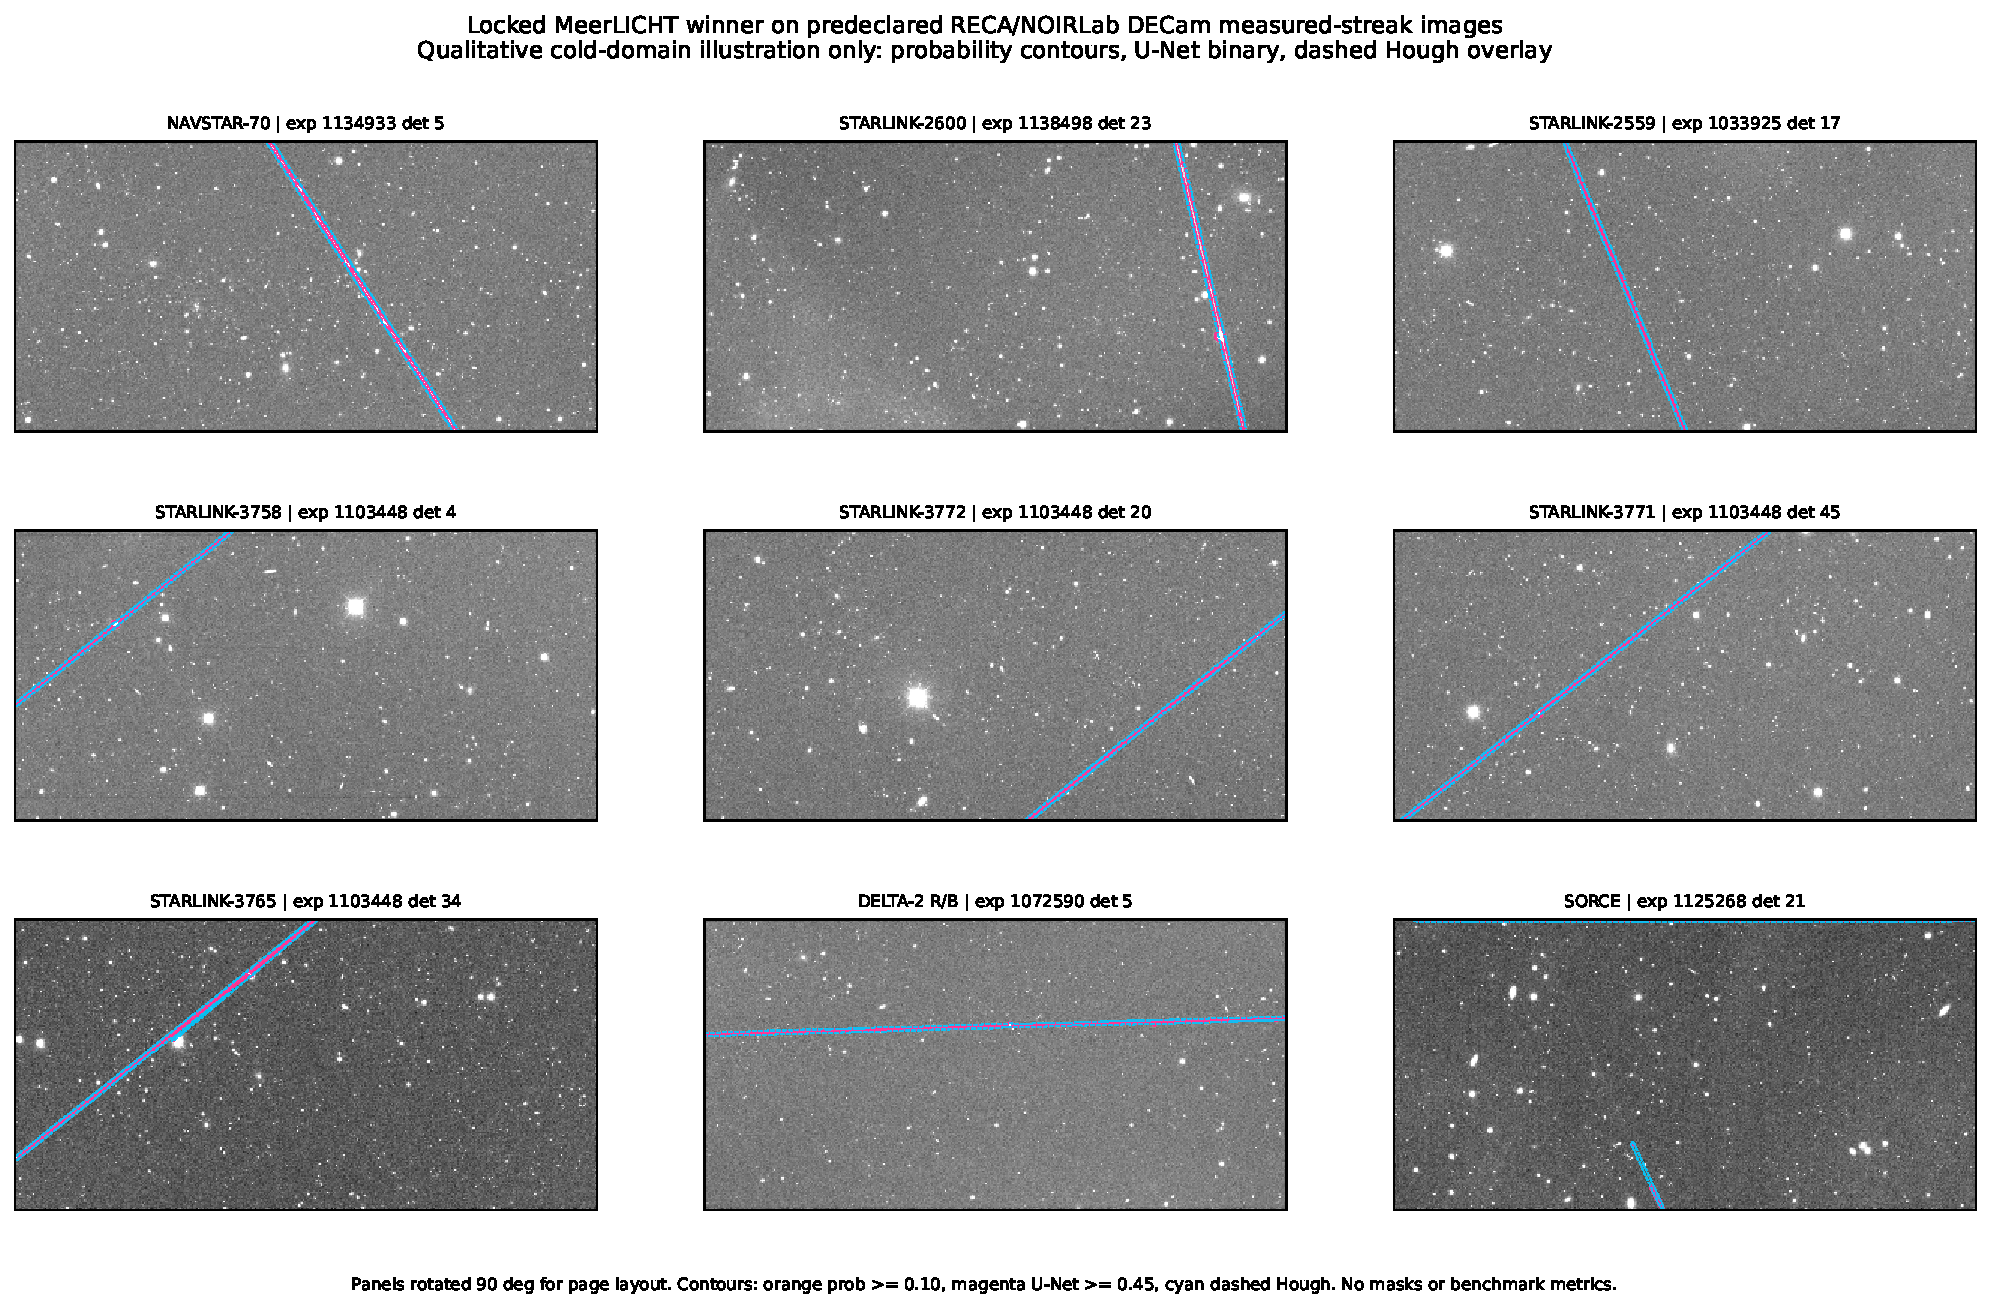
\includegraphics[width=\textwidth]{../results/figures/decam_cold_inference_montage.pdf}
  \caption{Locked MeerLICHT-trained U-Net applied cold to predeclared DECam
           measured-streak frames (panels rotated for layout; magenta: U-Net
           contour at $p\ge0.45$; cyan dashed: Hough). Qualitative illustration
           only: no ground-truth masks or benchmark metrics exist.}
  \label{fig:decam_cold_montage}
\end{figure}

%% ----- Residual error localisation (the core finding) -----
\section{Diagnostics localise much of the strict precision gap near the boundary}
\label{sec:ext_error}

The diagnostics below separate location from cause: most false-positive mass is
in trail-bearing patches, and the distance analysis shows that a majority of
false-positive pixels lie within one pixel of labelled trails. This is consistent
with thin or imperfect mask boundaries, while a smaller whole-patch component
remains genuine background confusion. Section~\ref{sec:ext_reannotation} tests
this reading against a blinded single-author re-annotation.

\subsection{False-positive decomposition}
\label{sec:ext_fpdecomp}

Decomposing the false-positive pixels of the winning model shows that only
$17.5\,\%$ are inter-patch (the network lighting up in trail-free patches), while
$82.5\,\%$ are intra-patch (falling inside trail-bearing patches, though not
necessarily adjacent to the trail) (Table~\ref{tab:fp_decomposition}). A patch-level gate addresses only the
inter-patch share, so this $17.5\,\%$ is a hard upper bound for such a gate;
hard-negative mining retrains and is only loosely bounded by it.

\begin{table}[htbp]
  \centering
  \caption{Decomposition of false-positive pixels. Only the inter-patch
           component is directly removable by a patch-level gate (a looser
           reference for hard-negative mining).}
  \label{tab:fp_decomposition}
  \begin{tabular}{lrr}
    \toprule
    Component & Pixels & Share \\
    \midrule
    Intra-patch FP & 300{,}745 & 82.5\% \\
    Inter-patch FP & 63{,}662 & 17.5\% \\
    \bottomrule
  \end{tabular}
\end{table}

\subsection{Boundary-tolerant evaluation}
\label{sec:ext_boundary}

Re-scoring under a symmetric boundary tolerance of $k\in\{0,1,2,3\}$\,px (RECT
structuring element; a predicted pixel within $k$\,px of ground truth counts
towards precision, and a ground-truth pixel within $k$\,px of a prediction
counts towards recall) isolates boundary disagreement from genuine misses
(Figure~\ref{fig:boundary_tolerance}). Allowing a single pixel of tolerance, the
five-seed mean precision rises from $0.847$ (strict) to $0.946$, recall from
$0.923$ to $0.980$, and the $\pm1$\,px $F_1$ reaches $0.962$: the precision gap
to the paper largely closes under a one-pixel tolerance. A one-sided check separates this from a
recall-for-precision trade: re-scoring the same predictions against ground
truth dilated by one pixel raises precision from $0.852$ to $0.937$ but drops
recall to $0.793$, whereas the symmetric tolerance raises both. This is
consistent with residual error dominated by boundary placement rather
than spurious detection. The blinded re-annotation of
Section~\ref{sec:ext_reannotation} supports this reading, and the tolerant score
is not treated as equivalent to the paper's strict $0.94/0.94$.

\begin{figure}[htbp]
  \centering
  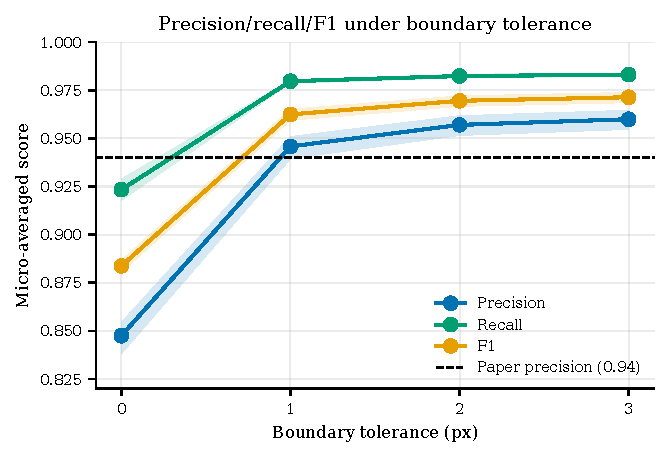
\includegraphics[width=0.85\textwidth]{../results/figures/thesis_2_boundary_tolerance.pdf}
  \caption{Boundary-tolerant metrics versus tolerance $k$ (micro-averaged);
           the horizontal line marks the paper's strict precision of $0.94$.
           One pixel of tolerance largely closes the strict gap, but the
           relaxed score is not directly comparable to the paper's strict
           metric.}
  \label{fig:boundary_tolerance}
\end{figure}

\subsection{False-positive distance to mask}
\label{sec:ext_fpdist}

The distance from each false-positive pixel to the nearest ground-truth trail
pixel concentrates at small values (Figure~\ref{fig:fp_distance}). Of all false
positives, $57\,\%$ lie within $1$\,px; of the distance-defined false positives
(those in trail-bearing patches, excluding the $\sim$$17\,\%$ whole-patch false
positives that have no defined distance), $69\,\%$ lie within $1$\,px, with a
median of $1.6$\,px. Both denominators are reported because the $69\,\%$ figure
alone overstates the global picture. The distribution is consistent with a
boundary-placement-dominated residual error plus a bounded genuine-background
minority.

\begin{figure}[htbp]
  \centering
  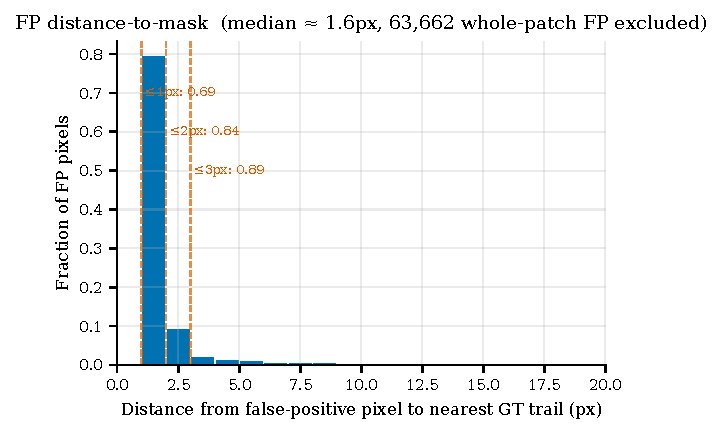
\includegraphics[width=0.85\textwidth]{../results/figures/ext_1_fp_distance_histogram.pdf}
  \caption{Cumulative fraction of distance-defined false-positive pixels within
           distance $d$ of the nearest ground-truth trail. The plotted curve
           excludes $63{,}662$ whole-patch FP pixels; $69.3\,\%$ of
           distance-defined and $57.2\,\%$ of all FP pixels lie within $1$\,px.}
  \label{fig:fp_distance}
\end{figure}

\subsection{Relative display-contrast diagnostics}
\label{sec:ext_faint}

The locked winner was rescored post hoc on the 31 positive test images using
raw 8-bit PNG intensities as a \emph{relative display-contrast proxy}, not
calibrated flux or signal-to-noise (Appendix
Figures~\ref{fig:faint_streak}--\ref{fig:fp_intensity}); median cross-sections
through labelled trails make the proxy concrete
(Figure~\ref{fig:faint_profiles}), and fitting calibrated flux in an aperture
would need counts the 8-bit renders do not carry (Section~\ref{sec:meerlicht}).
Across 55 cleaned trail components, the low-contrast tertile has the lowest
pre-Hough recall ($0.853$) and the largest Hough-added ground-truth fraction
($0.092$), with post-Hough recall at least $0.945$ in every tier, so Hough adds
most in the low-contrast tier where the network evidence is weakest. Near-trail false positives sit at
intermediate display excess between background and labelled-trail pixels
(Figure~\ref{fig:fp_intensity}): consistent with mask under-coverage near
labels and trail-like background further away, and descriptive rather than
evidence of label error.

\subsection{Topology-aware comparison (clDice)}
\label{sec:ext_cldice}

The centreline Dice (clDice) tracks pixel Dice and preserves the architecture
ordering: $0.847$ for the base model versus $0.838$ for the attention variant
($-0.009$), against pixel Dice $0.884$ and $0.879$ ($-0.005$). Topology
therefore agrees with the null attention result and shows no hidden connectivity
advantage.

\subsection{Blinded re-annotation audit}
\label{sec:ext_reannotation}

The diagnostics above localise the residual error but leave two explanations:
visible trails may be wider than the consortium masks, or the model may
systematically over-paint. To separate these, a blinded single-author,
evaluation-only re-annotation was performed on $64$ sealed $528\times528$
crops: crop identities were shuffled, and the original masks, predictions, and
crop--frame mapping remained sealed until the new masks and verdicts passed
validation. The sample covered interior and endpoint segments for boundary
scoring, plus false-positive-prone and quiet decoy patches as existence
controls, stratified by display contrast.

The audit does not support a systematic width bias. The original MeerLICHT
masks, the blinded re-annotation, and the model prediction all have median
stroke width $6$\,px. Per-crop width differences are centred near zero:
re-annotation minus original is $+0.10$\,px ($95\%$ CI $[-0.30,+0.53]$), and
model minus re-annotation is $+0.22$\,px ($[-0.09,+0.54]$). The strict
false-positive gap therefore cannot be explained simply by labels being
uniformly too thin or by the model being uniformly too wide.

Pixel agreement gives the same strict-tolerance picture. Over the $44$ interior
and endpoint crops, the model matches the re-annotation ($F_1=0.893$) about as
closely as the original consortium labels do ($0.890$), while the model and
consortium labels score $0.894$ against each other
(Table~\ref{tab:reannotation}, pixel-weighted micro-averages). A paired per-crop
bootstrap ($B=10{,}000$, equal weight per crop) puts the strict
model-minus-consortium difference against the re-annotation at $-0.0001$
($95\%$ CI $[-0.024,+0.022]$). At $\pm1$\,px the
model is marginally lower ($\Delta=-0.015$, CI $[-0.038,+0.003]$, just spanning
zero). Because the model was trained on the consortium labels, this is not
independent confirmation of the model; it shows that this audit detects no
statistically resolved strict excess over the original-label comparison under
this design. The
pattern is stable across strata, with median widths of $6$\,px and strict
$F_1$ near $0.86$ on interior segments and $0.89$ on endpoints.

The controls leave a small reference-relative over-firing residual. The model
detects signal on all $11$ false-positive-prone controls, while the
re-annotation marks a trail on only $5$; on the six over-fired crops the median
extra area is $134$\,px, about $0.05\,\%$ of a crop. The quiet decoys draw no
model detections. Figure~\ref{fig:supp_gold_audit} shows representative
overlays, and Figure~\ref{fig:supp_gold_audit_process} documents the sealed-crop
annotation process. The audit remains bounded by its design: a single,
dataset-familiar annotator estimates between-source disagreement rather than
inter-annotator agreement. Its value is therefore directional: it tests whether
a large width mismatch is visible, not what the unique true mask should be. A
multi-annotator gold standard remains the strongest remaining check
(Section~\ref{sec:future}).

\begin{table}[htbp]
  \centering
  \caption{Blinded re-annotation audit: micro-averaged strict and $\pm1$\,px
           $F_1$ over the $44$ interior and endpoint crops. All three sources
           share a median stroke width of $6$\,px.}
  \label{tab:reannotation}
  \begin{tabular}{lrr}
    \toprule
    Comparison & strict $F_1$ & $\pm1$\,px $F_1$ \\
    \midrule
    Consortium labels vs re-annotation & 0.890 & 0.978 \\
    Model vs re-annotation             & 0.893 & 0.970 \\
    Model vs consortium labels         & 0.894 & 0.972 \\
    \bottomrule
  \end{tabular}
\end{table}

%% ----- Model variants as tests of the error diagnosis -----
\section{Model variants under stated protocols}
\label{sec:ext_arch}

The model variants test the error diagnosis. If the precision gap were
dominated by empty-patch false positives, a patch classifier or hard-negative
training should give a material precision gain; if by missing faint structure,
attention gates might improve overlap or topology. The observed results are
narrower: the gate shifts precision in a direction consistent with the
$17.5\,\%$ inter-patch bound, and attention does not improve the base
architecture.

\subsection{Classifier-gated detector}
\label{sec:ext_twostage}

The classifier-gated detector (gate architecture and training in
Section~\ref{sec:classifier}) is reported descriptively as an
operating-characteristic Pareto front over the classifier and U-Net thresholds
(Figure~\ref{fig:two_stage_pareto}), not as a single selected replacement for the
locked U-Net. The gate suppresses only empty-patch false positives, so its
gain is bounded by the inter-patch share. At the illustrative high-recall operating point used for
Figure~\ref{fig:two_stage_pareto} ($t_{\mathrm{clf}}=0.18$,
$t_{\mathrm{U\mbox{-}Net}}=0.45$), the gate routes $2{,}625$ patches to the
U-Net ($75.3\,\%$ of the sampled test set), improving precision from $0.852$ to
$0.864$ while reducing recall from $0.918$ to $0.914$ and giving Dice $0.888$.
End-to-end recall counts classifier-rejected positive patches as false
negatives, exposing the classifier false-negative rate ($0.096$ at this
operating point) as a hard recall ceiling. The gate gives a bounded precision
gain (the $+1.2$\,pp shift is about one five-seed precision SD) and a real
compute saving at this operating point, but not an
order-of-magnitude saving: it skips $24.7\,\%$ of sampled-test U-Net forwards.
Larger savings would require a more aggressive gate on a denser, naturally
empty-dominated patch stream.

\begin{figure}[htbp]
  \centering
  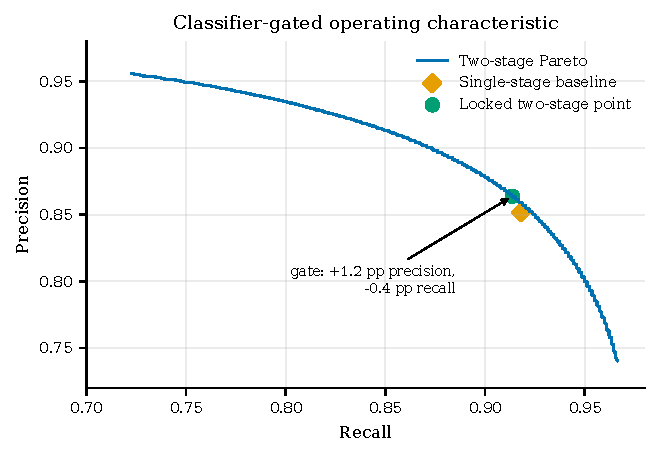
\includegraphics[width=0.8\textwidth]{../results/figures/thesis_5_two_stage_pareto.pdf}
  \caption{Two-stage operating-characteristic Pareto front over the
           classifier and U-Net thresholds; test-side and descriptive, not a
           validated improvement. The annotated point shifts precision
           $+1.2$\,pp and recall $-0.4$\,pp versus the locked baseline.}
  \label{fig:two_stage_pareto}
\end{figure}

\subsection{Attention-gated U-Net}
\label{sec:ext_attention}

Under a matched protocol (the balanced sweep, top-five five-seed retraining,
and validation-only selection of Section~\ref{sec:optuna}), the
attention-gated U-Net \citep{oktay2018} does not improve on
the base network despite carrying roughly $1\,\%$ more parameters. Its winner
(trial~7, selected over the marginally higher trial~35 by the same
lower-batch-size tie-breaker) reaches test precision $0.838$, recall $0.924$,
and Dice $0.879$ at threshold $0.48$, against the base Dice of $0.884$
(Table~\ref{tab:base_vs_attention}). The five-seed validation-restudy means are
$0.854$ for the base model ($90\,\%$ interval $[0.851,\,0.856]$) and $0.851$ for
the attention model ($[0.850,\,0.852]$), so the comparison is best read as
matched-protocol null evidence rather than as a decisive architectural ranking.
Together with the clDice result (Section~\ref{sec:ext_cldice}), the attention variant
reveals no hidden connectivity or faint-trail advantage on this dataset.
Supplementary Figure~\ref{fig:fp_fn_gallery_attn} shows the corresponding
false-positive/false-negative gallery for the attention model.

\begin{table}[htbp]
  \centering
  \caption{Five-seed test means for the base and attention-gated U-Nets.}
  \label{tab:base_vs_attention}
  \begin{tabular}{lrrr}
    \toprule
    Metric & Base U-Net mean & Attention U-Net mean & Delta \\
    \midrule
    Precision & 0.847 & 0.848 & +0.001 \\
    Recall    & 0.923 & 0.919 & -0.005 \\
    $F_1$     & 0.884 & 0.882 & -0.002 \\
    Dice      & 0.884 & 0.882 & -0.002 \\
    \bottomrule
  \end{tabular}
\end{table}

%% ----- Training protocol sensitivity -----
\section{Training and inference sensitivity}
\label{sec:ext_training}

\subsection{Data efficiency}
\label{sec:ext_dataeff}

Retraining the winning configuration on nested $30/50/70/100\,\%$ subsets of the
training images (validation and test held fixed) shows validation Dice flat to
$50\,\%$, rising at $70\,\%$, then near-constant
(Figure~\ref{fig:data_efficiency}). Because the hyperparameters are transferred
from the $100\,\%$-tuned winner rather than re-tuned per fraction, the curve is a
conservative estimate at each data size; it is a
single-seed, indicative result, plotted without a confidence band. The fixed
threshold-$0.5$ validation Dice values are $0.842$, $0.842$, $0.854$, and
$0.856$ for $30$, $50$, $70$, and $100\,\%$ of the training images,
respectively, so the main gain occurs before the final fraction. On this
single-seed curve the plateau suggests that the 178-image subset does not
obviously bind this architecture, which is consistent with the replication
reading of Section~\ref{sec:replication}.

\begin{figure}[htbp]
  \centering
  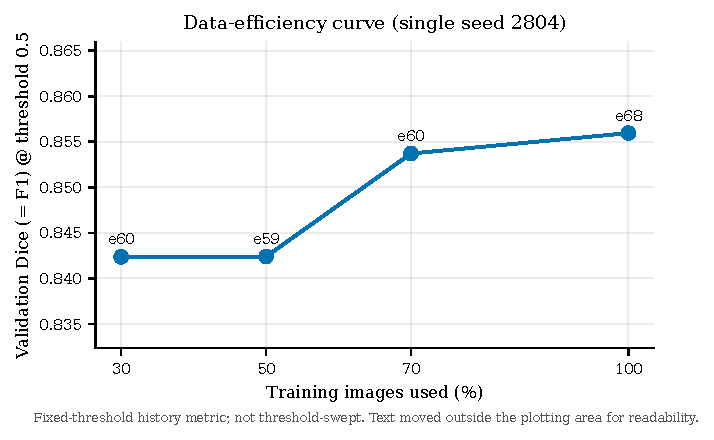
\includegraphics[width=0.8\textwidth]{../results/figures/thesis_4_data_efficiency.pdf}
  \caption{Validation Dice versus training-image fraction (single seed 2804;
           fixed-threshold history metric at $0.5$, not threshold-swept).
           Hyperparameters are transferred from the $100\,\%$ winner rather
           than re-tuned per fraction.}
  \label{fig:data_efficiency}
\end{figure}

\subsection{Hard-negative mining}
\label{sec:ext_hardneg}

Appending 150 mined hard-negative (false-positive empty) patches to the training
set yields a small precision gain in this single-seed confirmation: $+0.007$
precision ($0.852\rightarrow0.859$) at essentially unchanged recall ($-0.001$),
for $+0.003$ Dice. This $+0.007$ change is within the five-seed precision
dispersion ($\pm0.010$; Section~\ref{sec:bootstrap}), so it is directional
rather than a resolved gain, and is bounded by, and consistent with, the
$17.5\,\%$ inter-patch false-positive share.

\subsection{Soft-label (dilated-target) pilot}
\label{sec:ext_softlabel}

A single-seed pilot replacing the hard targets with $1$\,px dilated soft-edged
targets (training only; validation and test masks unchanged) improves no overlap,
precision or topology metric (Table~\ref{tab:soft_label}). The soft model predicts wider trails, with
its validation-optimal threshold rising from $0.45$ to $0.62$, giving recall
$+0.008$ but precision $-0.022$, exact Dice $-0.009$, clDice $-0.013$, and a
near-identical $\pm1$\,px $F_1$ ($-0.001$): the boundary band is absorbed into
wider predictions rather than sharpening localisation. The pilot is reported as a null result,
consistent with the boundary-placement interpretation.

\begin{table}[htbp]
  \centering
  \caption{Soft-label (dilated-target) pilot versus the hard-label winner; a
           single-seed protocol variant with no metric gain. Both columns are
           canonical seed-2804 values, so the hard-label $\pm1$\,px $F_1$ here
           is the seed-2804 figure ($0.963$); the five-seed mean is $0.962$
           (Section~\ref{sec:ext_boundary}).}
  \label{tab:soft_label}
  \begin{tabular}{lrrr}
    \toprule
    Metric & Hard-label winner & Dilated-soft pilot & Delta \\
    \midrule
    Exact Dice  & 0.884 & 0.875 & -0.009 \\
    $\pm1$ px $F_1$ & 0.963 & 0.962 & -0.001 \\
    clDice      & 0.847 & 0.835 & -0.013 \\
    \bottomrule
  \end{tabular}
\end{table}

%% ----- Inference-time sensitivity -----
\subsection{Ensembling with test-time augmentation}
\label{sec:ext_ensemble}

A five-checkpoint ensemble with test-time augmentation reaches Dice $0.8885$
(precision $0.852$, recall $0.929$ at threshold $0.44$), against the single-model
$0.8836$. The $+0.005$ Dice improvement is comparable to the five-seed dispersion
of the single model, so it is not treated as a material gain.

\subsection{Probability-stratified Hough}
\label{sec:ext_probhough}

Replacing the binary Hough input with a probability-stratified canvas is a
clean null: pixel recall changes by $+0.00003$, the patch-level
false-negative rate is identical, and Hough false-positive pixels rise from
$2{,}725{,}702$ to $2{,}785{,}274$. The locked binary Hough already recovers
essentially all recoverable pixels, so stratification only adds false
positives.

%%%%%%%%%%%%%%%%%%%%%%%%%%%%%%%%%%%%%%%%%%%%%%%%%%%%%%%%%%%%%%%%%%%%%%%%%%%%%%%%
%% CHAPTER 6 -- Discussion
%% Scope: deviations from the paper, limitations, and scientific implications.
%%%%%
\chapter{Discussion}
\label{ch:discussion}

\section{Deviations from the target paper}
\label{sec:deviations}

Faithful replication is a matter of degree, so Table~\ref{tab:deviations} makes
the remaining departures from \citet{stoppa2024} explicit. They are forced
choices where the paper omits training hyperparameters; deliberate methodology
choices such as image-level stratified splits, a validation-swept threshold, and
sampled-plus-parity testing; and implementation conventions such as the PyTorch
port and logits-with-external sigmoid output. Alignment only in spirit, as with
the squared-denominator Dice and stride-528 tiling, is not described as
paper-faithful.

\begin{table}[htbp]
  \centering
  \caption{Documented deviations from Stoppa et al.\ (2024).}
  \label{tab:deviations}
  \begin{tabular}{p{0.24\textwidth}p{0.34\textwidth}p{0.30\textwidth}}
    \toprule
    Aspect & This work & Target paper \\
    \midrule
    Framework & PyTorch & Keras / TensorFlow \\
    Architecture source & Reconstructed from the released Keras model,
      reimplemented in PyTorch & Released Keras model \\
    Output convention & Logits; sigmoid in loss/eval & Built-in final sigmoid \\
    Dice formulation & Squared-denominator (released ASTA code) & Standard Dice
      (paper text) \\
    Patch tiling & $528^2$ at stride $528$ ($20\times20$ grid) & $528^2$; tiling
      unspecified \\
    Threshold & Validation PR sweep ($F_1$-optimal) & Fixed $0.58$ \\
    Splits & Image-level, trail-pixel-stratified; $122/24/32$ & Not specified \\
    Test sampling & Sampled $1{:}3$ plus parity (all negatives) & 20{,}000-patch
      set \\
    Hough input & Patch-reconstructed; full-coverage parity & Dense full image \\
    Hyperparameters & Validation-only Optuna search & Not published \\
    Noise augmentation & Calibrated train-only signal-dependent noise & Not
      specified \\
    \bottomrule
  \end{tabular}
\end{table}

\noindent The swept threshold and different test population change the headline
comparison, chiefly by confounding precision and leaving recall as the closest
like-for-like quantity (Section~\ref{sec:replication}). The Hough comparison is
checked on a full-coverage canvas, but strict precision remains sensitive to the
$3$\,px line-rasterisation convention (Section~\ref{sec:hough_results}). The
remaining departures were not individually isolated: architecture tests lock the
framework port and output convention, image-level splitting removes patch-level
leakage, and calibrated noise was validation-screened before adoption.

\section{Interpreting the headline comparison}
\label{sec:interpretation}

Section~\ref{sec:deviations} leaves recall as the like-for-like quantity, and
even that spans different populations - the 32 test images here against the
paper's 20{,}000 patches of unreported class balance. For precision the prevalence
confound is measured, not assumed: the fall from $0.852$ to $0.780$ at identical
recall and fixed threshold is the direct size of the base-rate effect, while
Section~\ref{sec:ext_error} localises the annotation confound at about one pixel.
Evaluating at the paper's fixed $0.58$ rather than the swept $0.45$ raises
precision by only $0.025$, so the threshold is a minor contributor.

The Hough comparison is favourable for completeness but not for strict
precision: the same gain in pixel completeness (Section~\ref{sec:hough_results})
cuts strict pixel precision from $0.780$ to $0.410$, about half of which is
sensitive to the $3$\,px line-rasterisation convention in a line-thickness sweep
rather than necessarily reflecting genuine false detection
(Figure~\ref{fig:supp_hough_thickness}). On this full-coverage tiled canvas,
verified pixel-for-pixel against the parity canvas, this is comparable
completeness, not superiority. The same discipline
applies to the tolerant scores: the $\pm1$\,px precision $0.946$ locates the
residual at the boundary scale but is never set against the paper's strict
$0.94/0.94$, and these diagnostics hold across the five seeds
(Figure~\ref{fig:supp_multiseed}).

\section{Limitations}
\label{sec:limitations}

The findings above are bounded by seven limitations.

\begin{itemize}
  \item \textbf{Mask under-coverage.} The annotations occasionally omit
        faint endpoints and low-contrast stretches
        (Section~\ref{sec:mask_quality}). The effect is asymmetric: a correct
        detection of an unlabelled trail pixel scores as a false positive,
        and a model trained on such labels also learns to suppress faint
        extensions. Label-referenced precision is therefore a lower
        bound where masks omit visible trail pixels. The blinded re-annotation
        (Section~\ref{sec:ext_reannotation}) finds no systematic width difference
        from the labels; a multi-annotator audit would measure any residual
        under-coverage directly.
  \item \textbf{Dataset size.} The subset holds 178 images, of which 32 form
        the test set. Image-level bootstrap intervals are accordingly several
        times wider than patch-level ones (Section~\ref{sec:bootstrap}), the
        image-level detection rate saturates, and the protocol-sensitivity
        results (data efficiency, hard negatives, soft labels) are
        single-seed pilots.
  \item \textbf{Sampled evaluation distribution.} The sampled test set keeps
        a $1{:}3$ positive-to-negative patch prior, which inflates precision
        relative to the natural, roughly $93\,\%$-empty population; the
        parity evaluation restores the negatives but is still scored at the
        sampled-validation threshold. The sampled-to-parity precision drop
        ($0.852$ to $0.780$) bounds the size of this bias; recall is
        unaffected because all positive patches are retained.
  \item \textbf{Hough rasterisation convention.} The parity Hough canvas is a
        verified full-coverage tiled prediction, not a patch-sampling artefact; the
        one residual is the $3$\,px line-drawing convention, which accounts for
        about half of the post-Hough precision fall.
  \item \textbf{Single telescope.} All training and quantitative evaluation
        use MeerLICHT data; transfer to another instrument's pixel scale,
        point-spread function, or background is untested, and the DECam
        application (Figure~\ref{fig:decam_cold_montage}) is qualitative only.
        The DECam montage is therefore a transfer sanity check, not evidence of
        deployable cross-instrument performance.
  \item \textbf{PNG-only inputs.} The 8-bit renders cap the dynamic range
        and carry no WCS, exposure, or photometric headers. Trails near the
        display floor may be undetectable in principle, and the contrast
        statements of Section~\ref{sec:ext_faint} are display-space proxies.
        The direction of any bias is unclear, because the labels were drawn
        on the same renders.
  \item \textbf{Single-band imagery.} Each frame provides one display
        channel, so no claim extends to multi-band trail morphology
        \citep{yu2025}.
\end{itemize}

\section{Scientific implications}
\label{sec:implications}

The error characterisation carries three implications beyond this
replication, and a practical reading for deployment.

First, where masks omit visible trail pixels, strict label-referenced precision
is best read as a conservative estimate, and the Hough stage makes this concrete:
it extrapolates linear extent the network under-detects, but where the
annotation also omits that extent the recovered pixels score as false
positives - the metric can penalise the recovery the stage was built for.
Reported precision for this
detector family should therefore be read alongside a statement of label quality;
comparisons across papers with different annotation conventions conflate
detector quality with labelling convention.

Second, pixel-level false-negative rates have an instance-level blind spot: the
semantic formulation labels every trail pixel identically, so two near-parallel
trails merged into one detection lose nothing under any pixel metric here.
Freshly launched constellation ``trains'' produce precisely this geometry, which
matters wherever downstream consumers need trail counts rather than masks.

Third, the boundary-placement finding suggests a practical reporting standard.
A majority of false-positive pixels lie within about one pixel of the labelled
boundary, no tested change resolves that residual, and the blinded re-annotation
(Section~\ref{sec:ext_reannotation}) is consistent with the reading that strict
performance is limited by annotation granularity. Evaluations of thin-artefact
detectors should therefore
record a mask-width convention and report a $\pm1$\,px boundary-tolerant
operating point alongside the strict score, so that boundary convention and
detection failure are separated rather than summed.

In practice, the decomposition reads as deployment guidance. Mask-dilation
before stacking would absorb a one-pixel boundary residual, so the
strict-precision gap may matter less for masking (untested). The classifier gate
is best treated as a compute feature - it skips $24.7\,\%$ of U-Net forwards,
more at natural prevalence - with precision headroom capped by the $17.5\,\%$
inter-patch share. Thresholds do not transfer across prevalence, so a deployed
detector should re-select its operating point at the deployment prevalence.


%%%%%%%%%%%%%%%%%%%%%%%%%%%%%%%%%%%%%%%%%%%%%%%%%%%%%%%%%%%%%%%%%%%%%%%%%%%%%%%%
%% CHAPTER 7 -- Conclusions and future work
%%%%%
\chapter{Conclusions and Future Work}
\label{ch:conclusions}

\section{Conclusions}
\label{sec:conclusions}

This dissertation replicated the \citet{stoppa2024} U-Net plus probabilistic
Hough satellite-trail detector on a 178-image MeerLICHT subset, with the
architecture recovered from the released model and the model and threshold
locked on validation data alone. The replication reproduces the paper's recall
closely (five-seed sampled-test recall $0.923\pm0.007$ against $0.94$, Dice
$0.884\pm0.004$) and its Hough completeness (trail-pixel recall $0.918\rightarrow0.990$
on the full-coverage parity canvas). Strict pixel precision sits below the
published level ($0.847$ sampled, $0.780$ at parity) and is prevalence-dependent,
leaving recall as the like-for-like comparison across test populations.

The follow-up analyses localise the precision gap rather than merely reporting
it: a one-pixel boundary tolerance raises five-seed precision from $0.847$ to
$0.946$, and $57\,\%$ of false positives lie within one pixel of a labelled
trail. A blinded single-author re-annotation then tests the main ambiguity: the
original labels, the re-annotation, and the model all have median width $6$\,px,
with no systematic width bias and no statistically resolved strict excess over
the original-label comparison under this design. The tested
interventions - classifier gate, attention U-Net, data efficiency,
hard-negative mining, soft labels, ensembling, and probability-stratified
Hough - are small or null under their stated protocols. The null variants still
matter: they close off obvious capacity and protocol explanations without making
the boundary diagnosis decisive. None resolves the residual materially, so
boundary-placement remains the most consistent reading.

The project also demonstrates a methodology. Faithful replication - architecture
recovered from released weights, preregistered selection, and sampled-versus-parity
evaluation kept distinct - surfaced at each step a discrepancy a looser
reproduction would have absorbed into an unexplained shortfall. Treating the
remaining gap as an object of analysis converted a headline deficit into a
measured, bounded mechanism. Conducted at this fidelity, replication is not a
re-implementation exercise but an instrument for locating where a published
result's accuracy resides: in the detector, in the labels, or in the metric.

\section{Future work}
\label{sec:future}

Several directions follow. The strongest remaining check is a \emph{multi-annotator
gold-standard audit}: independent annotators would establish inter-annotator
agreement and convert the single-author between-source estimate
(Section~\ref{sec:ext_reannotation}) into an agreement-bounded estimate of how
much of the strict precision gap is mask granularity rather than detector error.
A second priority is a \emph{labelled cross-instrument evaluation} - the DECam
application here is qualitative only (Figure~\ref{fig:decam_cold_montage}) - with
a classical baseline in the spirit of \citet{serrano2026}, on which attention
\citep{oktay2018} and richer architectures could be re-examined where the
matched-capacity null may not persist.

Secondary directions follow from the metric's instance-level blindness. An
\emph{instance-level} detection score over matched trail instances would expose
the merged near-parallel-trail failure mode that pixel rates cannot register,
made quantitative by a synthetic constellation-``train'' probe. Trail
\emph{removal} - combining the detected mask with the fitted Hough geometry to
interpolate across the trail - is the natural downstream step, though on 8-bit
renders this is cosmetic reconstruction rather than photometric recovery.

%%%%%%%%%%%%%%%%%%%%%%%%%%%%%%%%%%%%%%%%%%%%%%%%%%%%%%%%%%%%%%%%%%%%%%%%%%%%%%%%
%% Bibliography
%%%%%
\cleardoublepage
\phantomsection
\addcontentsline{toc}{chapter}{Bibliography}
\bibliographystyle{plainnat}
\bibliography{thesis}

%%%%%%%%%%%%%%%%%%%%%%%%%%%%%%%%%%%%%%%%%%%%%%%%%%%%%%%%%%%%%%%%%%%%%%%%%%%%%%%%
%% Appendices
%%%%%
\appendix

\chapter{Hyperparameter Search Space}
\label{app:hparam}

Table~\ref{tab:hparam_space} records the Optuna search space; all other
training choices are fixed by the methodology in Chapter~\ref{ch:pipeline}.

\begin{table}[htbp]
  \centering
  \caption{Optuna hyperparameter search space.}
  \label{tab:hparam_space}
  \small
  \begin{tabular}{p{0.22\textwidth}p{0.18\textwidth}p{0.22\textwidth}p{0.26\textwidth}}
    \toprule
    Parameter & Type & Range / values & Notes \\
    \midrule
    \texttt{learning\_rate} & log-uniform & $[10^{-4},\,10^{-3}]$ & Common range
      for all batch sizes \\
    \texttt{bce\_weight} & uniform & $[0.2,\,0.8]$ &
      $\lambda_{\mathrm{Dice}}=1-\lambda_{\mathrm{BCE}}$ \\
    \texttt{batch\_size} & fixed allocation & $\{8,16,32\}$ & 45 trials total;
      15 per batch size \\
    \bottomrule
  \end{tabular}
\end{table}


\chapter{Supplementary Results}
\label{app:supplementary}

\section{Post-hoc Trail and Error Diagnostics}
\label{app:posthoc_diagnostics}

\begin{figure}[htbp]
  \centering
  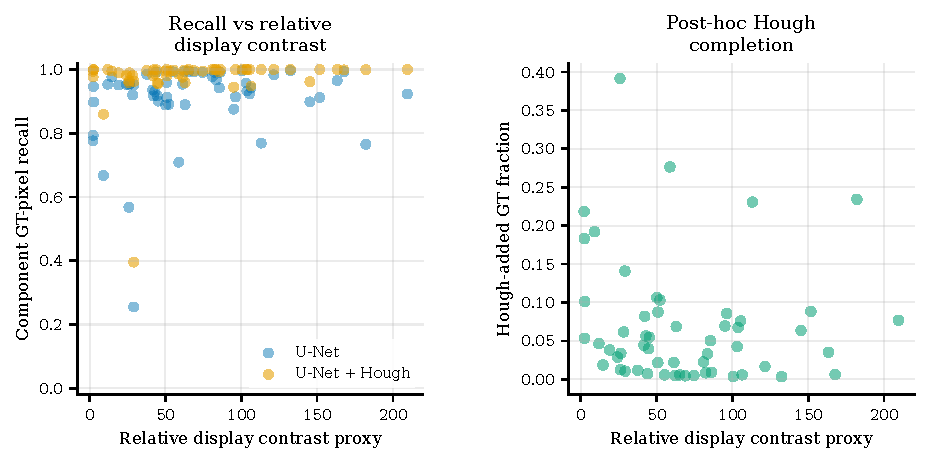
\includegraphics[width=0.9\textwidth]{../results/figures/faint_streak_contrast_vs_recall.pdf}
  \caption{Relative display contrast versus U-Net recall and Hough completion
           for the locked winner; the contrast proxy is descriptive, not
           calibrated flux or SNR.}
  \label{fig:faint_streak}
\end{figure}

\begin{figure}[htbp]
  \centering
  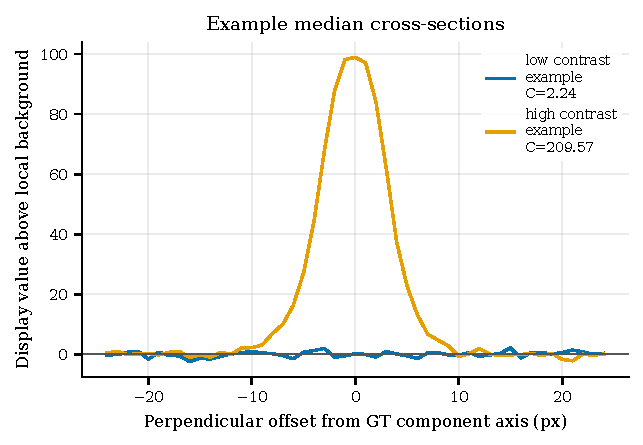
\includegraphics[width=0.9\textwidth]{../results/figures/faint_streak_profiles.pdf}
  \caption{Median cross-sections through labelled trails in display-space PNG
           values; descriptive examples of the relative-contrast proxy.}
  \label{fig:faint_profiles}
\end{figure}

\begin{figure}[htbp]
  \centering
  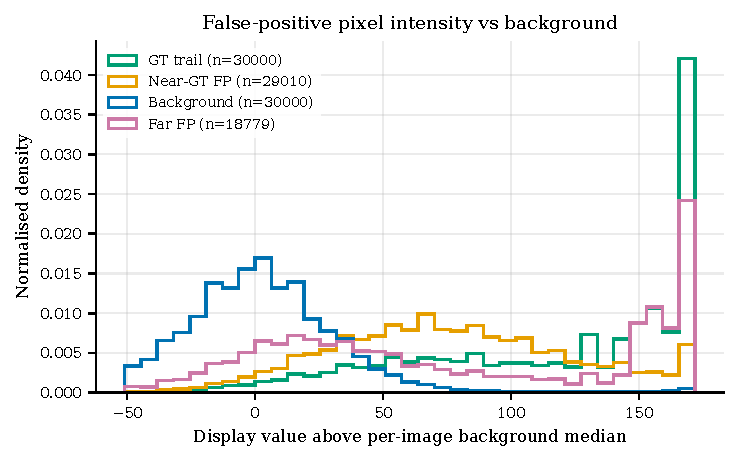
\includegraphics[width=0.9\textwidth]{../results/figures/fp_intensity.pdf}
  \caption{False-positive pixel display intensity versus labelled trail and
           background pixels. The KS distances are consistent with mask
           under-coverage and background confusion, but remain descriptive.}
  \label{fig:fp_intensity}
\end{figure}

\begin{figure}[htbp]
  \centering
  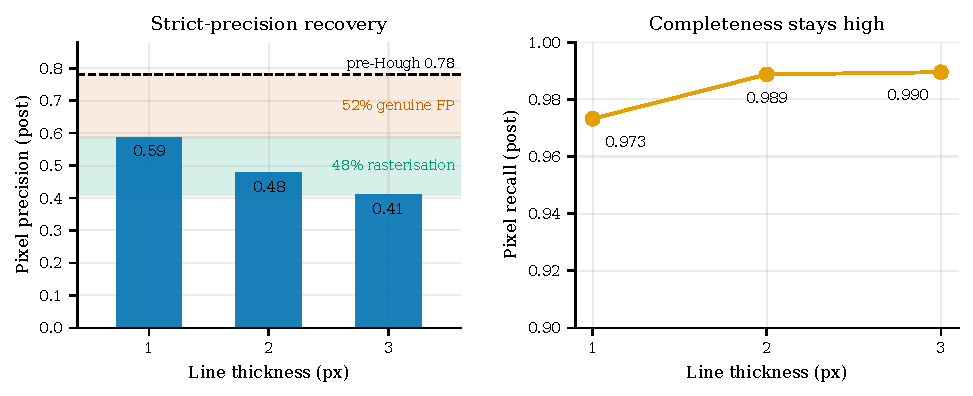
\includegraphics[width=0.9\textwidth]{../results/figures/supp_1_hough_thickness_recovery.pdf}
  \caption{Post-Hough strict pixel precision (left) and completeness (right) on
           the parity canvas as the drawn Hough line thickness varies over
           $1$--$3$\,px. Thinning the line from $3$ to $1$\,px recovers roughly
           half of the $0.780\rightarrow0.410$ precision fall while completeness
           stays above $0.97$, consistent with about half the fall arising from
           the $3$\,px rasterisation convention over the roughly $6$\,px masks
           and the remainder not being recovered by $1$\,px line thinning.}
  \label{fig:supp_hough_thickness}
\end{figure}

\begin{figure}[htbp]
  \centering
  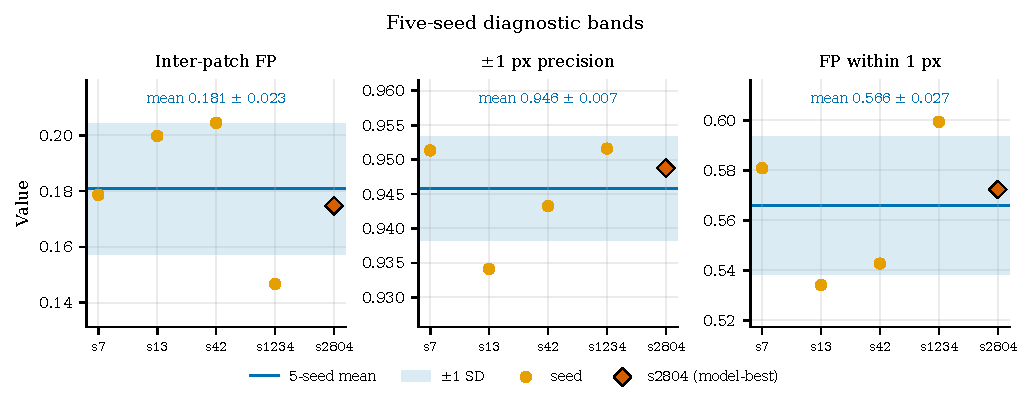
\includegraphics[width=0.9\textwidth]{../results/figures/supp_2_diagnostics_multiseed_bands.pdf}
  \caption{The three load-bearing boundary diagnostics across the five
           retraining seeds: inter-patch false-positive share, $\pm1$\,px
           precision, and false positives within $1$\,px. Markers are per-seed
           values; the line and shaded band give the five-seed mean $\pm1$\,SD;
           the diamond marks the locked winner (seed $2804$, \texttt{model-best}),
           which lies inside every band.}
  \label{fig:supp_multiseed}
\end{figure}

\begin{figure}[htbp]
  \centering
  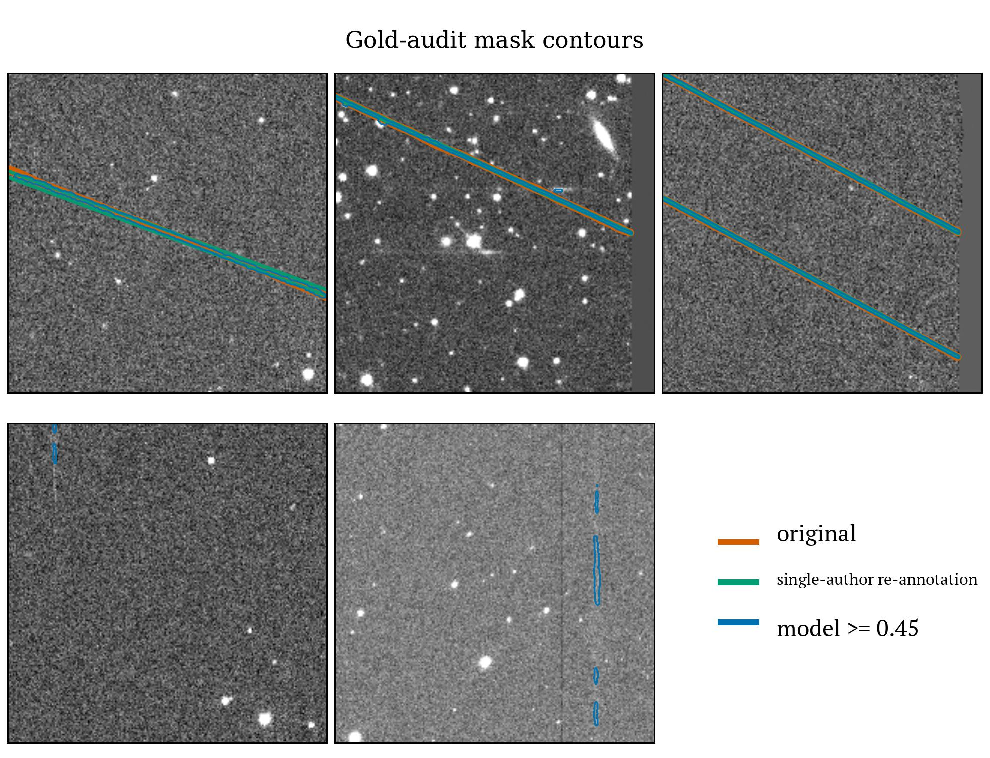
\includegraphics[width=0.9\textwidth]{../results/figures/supp_3_gold_audit_overlays.pdf}
  \caption{Blinded re-annotation overlays for five audit crops. Contours show
           the original MeerLICHT mask (orange), the blinded single-author
           re-annotation (green), and the locked model prediction at threshold
           $0.45$ (blue). The fixed selection shows the three lowest-index
           non-empty interior/endpoint crops, where boundaries are
           near-coincident, and the two lowest-index false-positive-prone
           controls with model-only over-firing. The single-author
           re-annotation is not an independent gold standard.}
  \label{fig:supp_gold_audit}
\end{figure}

\begin{figure}[htbp]
  \centering
  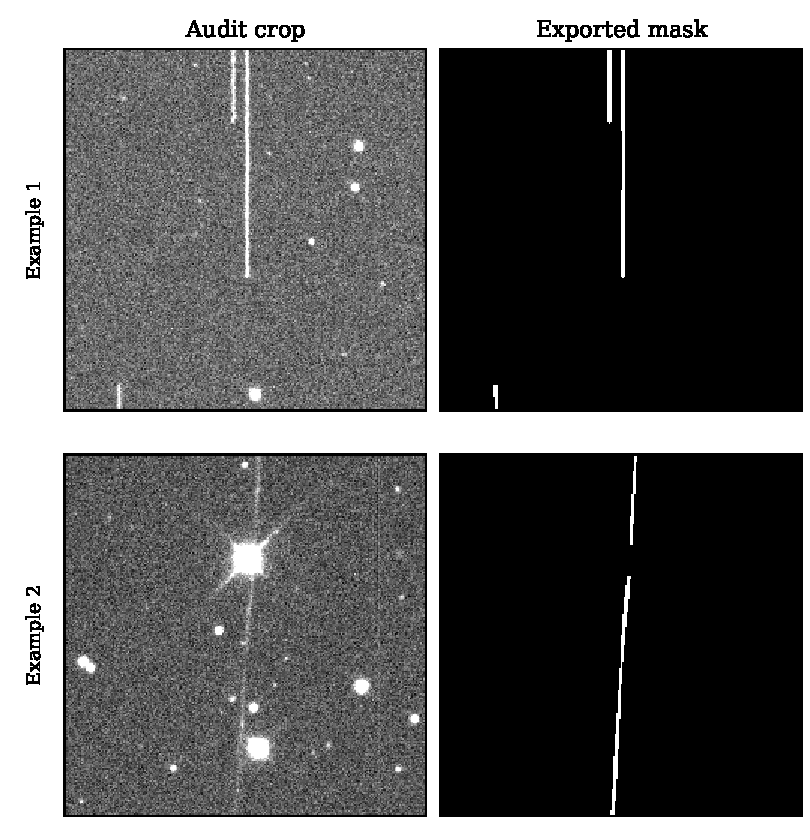
\includegraphics[width=0.72\textwidth]{../results/figures/supp_4_gold_audit_annotation_examples.pdf}
  \caption{Illustrative crop--mask pairs from the blinded re-annotation audit.
           Left: sealed audit crops before annotation; right: exported binary
           re-annotation masks. The full private gold set is not redistributed.
           Re-annotations were drawn in GIMP at fixed $400\%$ zoom with no
           per-crop contrast adjustment, using the Pencil tool with a $1$\,px
           hard edge, $100\%$ hardness, $100\%$ opacity, and dynamics off, then
           exported as binary 0/255 PNG masks.}
  \label{fig:supp_gold_audit_process}
\end{figure}

\clearpage
\section{Prediction Galleries}
\label{app:prediction_galleries}

\begin{figure}[htbp]
  \centering
  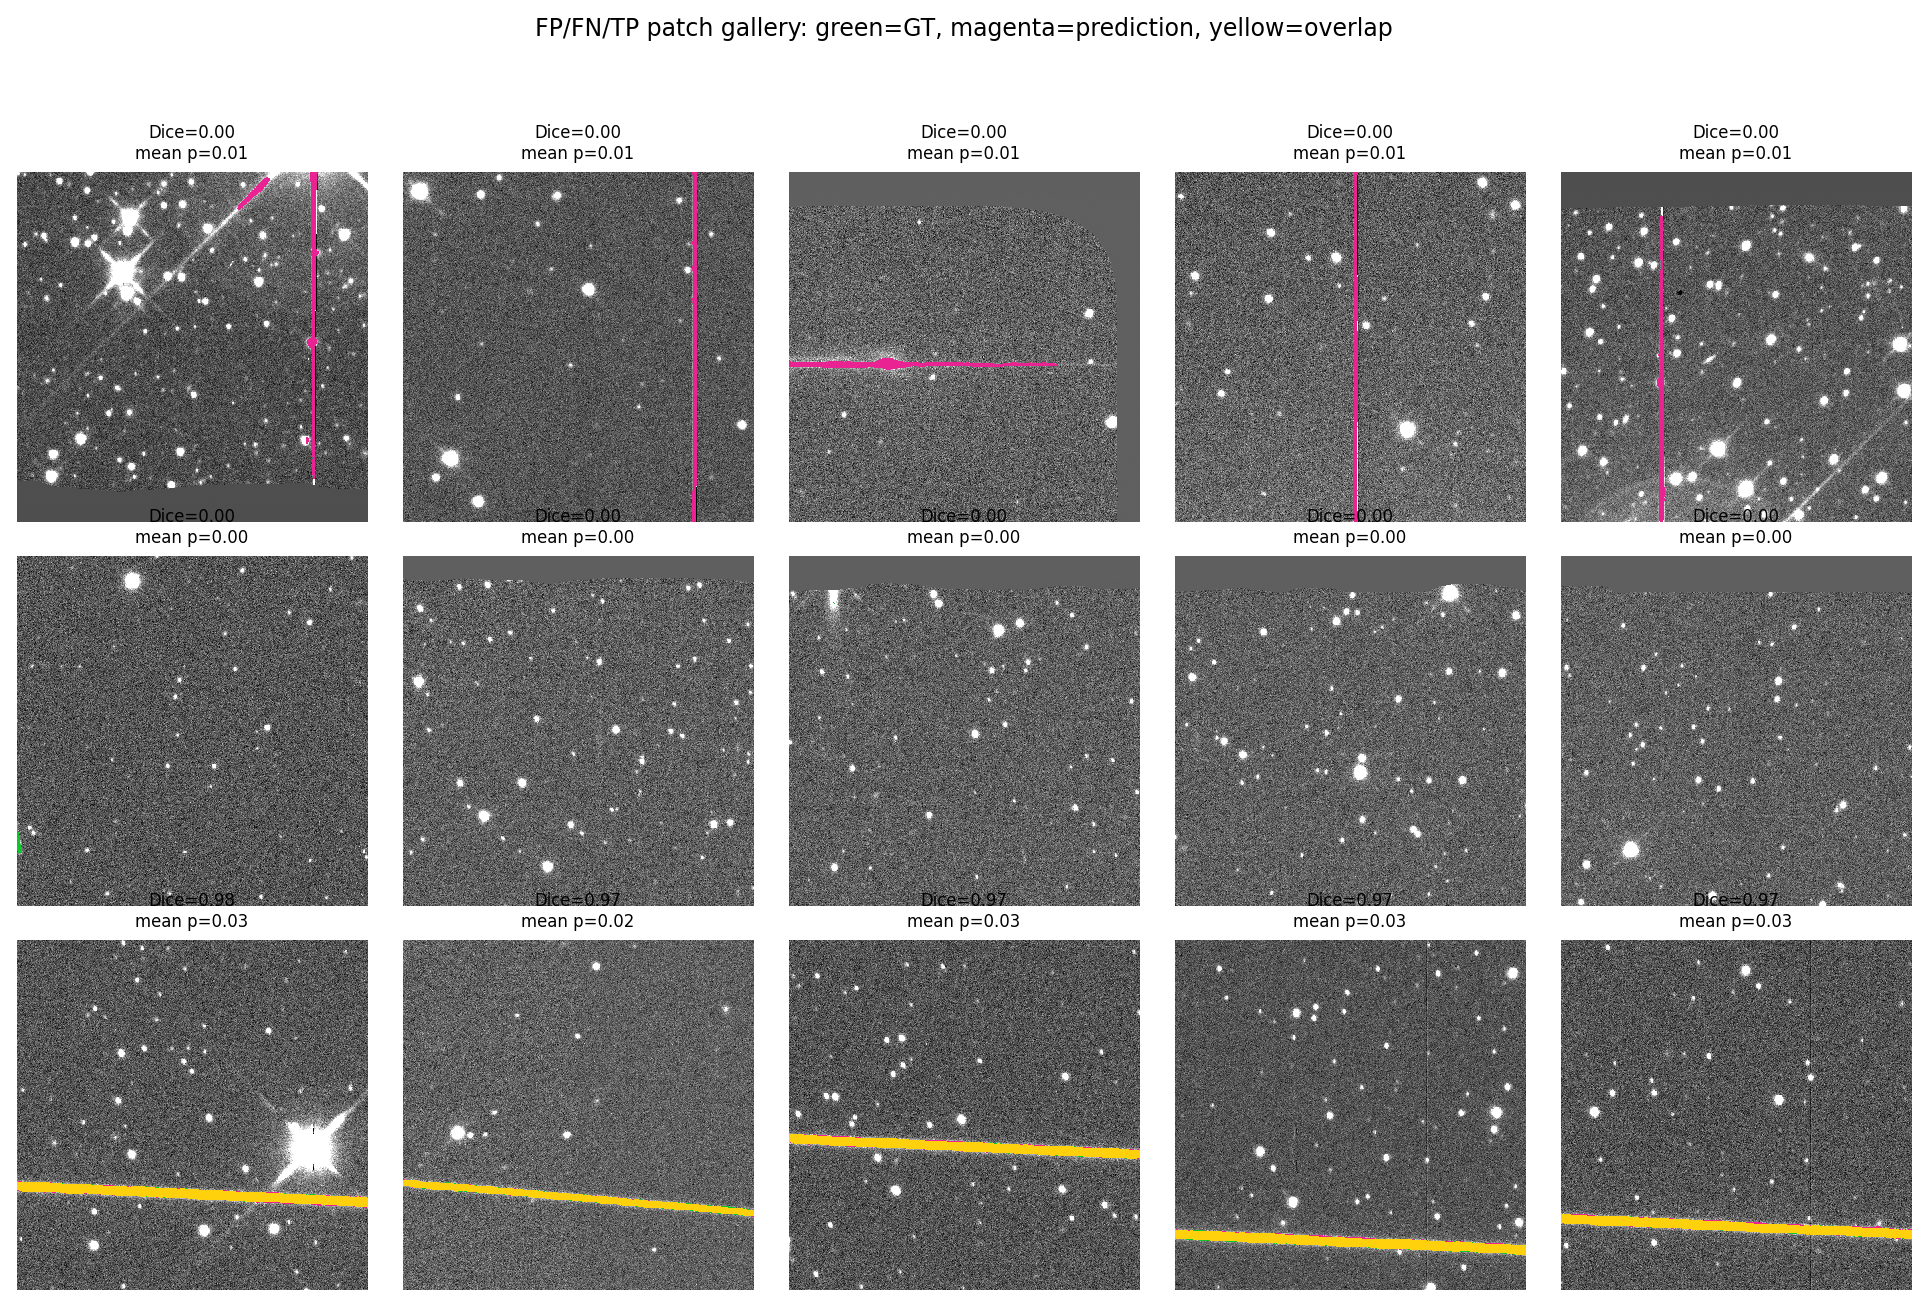
\includegraphics[width=\textwidth]{../results/figures/predictions/fp_fn_gallery_winner_t44_s2804.png}
  \caption{False-positive and true-positive gallery for the locked winner,
           including bright-star diffraction-spike examples alongside high-Dice
           cases where bright stars are correctly ignored.}
  \label{fig:fp_fn_gallery_winner}
\end{figure}

\begin{figure}[htbp]
  \centering
  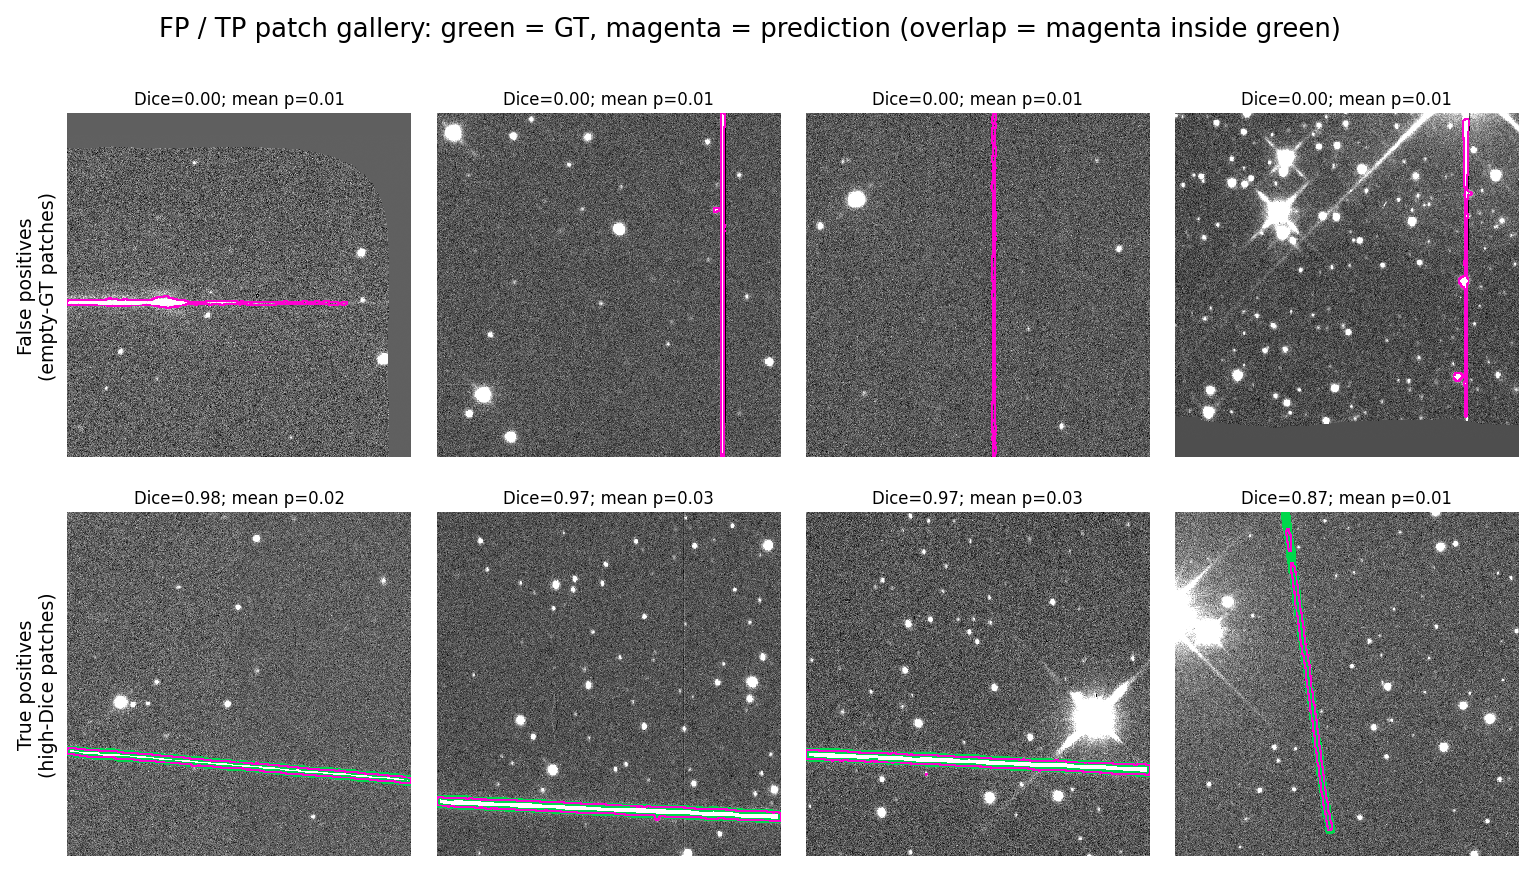
\includegraphics[width=\textwidth]{../results/figures/predictions/fp_fn_gallery_attn_winner_t7_s2804.png}
  \caption{The same eight patches for the attention-gated U-Net, in the order
           of Figure~\ref{fig:fp_fn_gallery_winner}, each with that model's own
           segmentation and Dice score.}
  \label{fig:fp_fn_gallery_attn}
\end{figure}

\chapter{Use of Auto-generation Tools}
\label{app:autogen}

I have used Codex (ChatGPT) and Claude Code to support me across this work,
primarily in the following areas:
\begin{itemize}
  \item Providing advice and usage support for libraries like PyTorch and PIL.
  \item Generating boilerplate code for plotting, testing and scripting.
  \item Generating function docstrings.
  \item Reviewing and auditing project structure for completeness, consistency,
        accuracy and best practices in software engineering.
\end{itemize}

\end{document}
